% Use only LaTeX2e, calling the article.cls class and 12-point type.

\documentclass[12pt]{article}

% Users of the {thebibliography} environment or BibTeX should use the
% scicite.sty package, downloadable from *Science* at
% www.sciencemag.org/about/authors/prep/TeX_help/ .
% This package should properly format in-text
% reference calls and reference-list numbers.

\usepackage{scicite}

% Use times if you have the font installed; otherwise, comment out the
% following line.

\usepackage{times}

% The preamble here sets up a lot of new/revised commands and
% environments.  It's annoying, but please do *not* try to strip these
% out into a separate .sty file (which could lead to the loss of some
% information when we convert the file to other formats).  Instead, keep
% them in the preamble of your main LaTeX source file.

\usepackage{amsmath}
\usepackage{amssymb}
\usepackage{graphicx}
\usepackage{subfig}
\usepackage{indentfirst}

% The following parameters seem to provide a reasonable page setup.

\topmargin 0.0cm
\oddsidemargin 0.2cm
\textwidth 16cm 
\textheight 21cm
\footskip 1.0cm


%The next command sets up an environment for the abstract to your paper.

\newenvironment{sciabstract}{%
\begin{quote} \bf}
{\end{quote}}


% If your reference list includes text notes as well as references,
% include the following line; otherwise, comment it out.

\renewcommand\refname{References}

% The following lines set up an environment for the last note in the
% reference list, which commonly includes acknowledgments of funding,
% help, etc.  It's intended for users of BibTeX or the {thebibliography}
% environment.  Users who are hand-coding their references at the end
% using a list environment such as {enumerate} can simply add another
% item at the end, and it will be numbered automatically.

\newcounter{lastnote}
\newenvironment{scilastnote}{%
\setcounter{lastnote}{\value{enumiv}}%
\addtocounter{lastnote}{+1}%
\begin{list}%
{\arabic{lastnote}.}
{\setlength{\leftmargin}{.22in}}
{\setlength{\labelsep}{.5em}}}
{\end{list}}


% Include your paper's title here

\title{Dynamical Decomposition on Fast-folding Proteins and Intrinsically Disordered Proteins} 


% Place the author information here.  Please hand-code the contact
% information and notecalls; do *not* use \footnote commands.  Let the
% author contact information appear immediately below the author names
% as shown.  We would also prefer that you don't change the type-size
% settings shown here.

\author
{Wangfei Yang,$^{1,2}$ Lorenzo Boninsegna,$^{1,3}$ Wenwei Zheng$^{4}$ and Cecilia Clementi$^{1,3\ast}$\\
\\
\normalsize{$^{1}$Center for Theoretical Biological Physics, Rice University, Houston, TX 77005, USA}\\
%\normalsize{Houston, TX 77005, USA}\\
\normalsize{$^{2}$Systems, Synthetic and Physical Biology Program, Rice University, Houston, TX 77005, USA}\\
%\normalsize{6100 Main St. Houston, TX 77005, USA}\\
\normalsize{$^{3}$Department of Chemistry, Rice University, Houston, TX 77005, USA}\\
\normalsize{$^{4}$College of Integrative Sciences and Arts, Arizona State University, Mesa, AZ 85212, USA}\\
\\
\normalsize{$^\ast$To whom correspondence should be addressed; E-mail:  cecilia@rice.edu.}
}

% Include the date command, but leave its argument blank.

\date{\today}



%%%%%%%%%%%%%%%%% END OF PREAMBLE %%%%%%%%%%%%%%%%



\begin{document} 

% Double-space the manuscript.

\baselineskip24pt

% Make the title.

\maketitle 



% Place your abstract within the special {sciabstract} environment.

\begin{sciabstract}
  Biomacromolecules always contain a very large number of degrees of freedom in an atomic resolution. Finding a coarser representation which captures the long-timescale dynamics is significant for investigating the characteristics of the molecules and constructing an effective coarse-grained model for them. Recently a data-driven decomposition algorithm, {\it Structure and State Space Decomposition}, was proposed while it has only been applied on two proteins. Here, we apply this algorithm on a set of 10 fast-folding proteins to test its robustness. We also propose a modified version of this algorithm for intrinsically disordered proteins. The results from different proteins show a consistency. Interestingly, the results also show that the dynamical decomposition for a frustrated protein differs significantly from the results from good folders.
\end{sciabstract}

% In setting up this template for *Science* papers, we've used both
% the \section* command and the \paragraph* command for topical
% divisions.  Which you use will of course depend on the type of paper
% you're writing.  Review Articles tend to have displayed headings, for
% which \section* is more appropriate; Research Articles, when they have
% formal topical divisions at all, tend to signal them with bold text
% that runs into the paragraph, for which \paragraph* is the right
% choice.  Either way, use the asterisk (*) modifier, as shown, to
% suppress numbering.

\section*{Introduction}

Thanks to recent developments of our computational power, now we are able to perform molecular dynamics (MD) simulations for biomacromolecules of considerable size on a timescale of milliseconds, which is the typical timescale for biomolecular processes such as protein folding and ligand binding, with an atomic resolution\cite{DE_Shaw_fast-folding}. However, our computational power is still limited to allowing us to use the same method for larger systems or longer timescales. Fortunately, empirical results and theoretical researches indicate that for most biomacromolecular processes only a little part of the phase space is highly relevant, and the rest is just noise orthogonal to it. Thus, we can overcome the computational limitation by constructing a reduced model, {\it i.e.} coarse-grained (CG) model, which conserves the most ``interesting'' portion but wipes off the noise pretty much. To construct such a model, first we need to identify the subset of the phase space that is highly relevant to the processes we're interested in and the corresponding collective variables can be used as the representation for the reduced model. After that, we can define the effective atoms (CG beads) based on the collective variables.

Recently, a data-driven algorithm called {\it Structure and State Space Decomposition} (S3D) has been proposed by Boninsegna {\it et al} to obtain the collective variables from all-atom simulation data\cite{Lrenzo_S3D}. While only two proteins were tested with this decomposition algorithm in the original paper. We think that applications on more proteins are necessary to test the robustness of the algorithm itself, and we can also check if there are general patterns in the decomposition results and if the results from different proteins are consistent.

We here applied S3D algorithm on a set of 10 fast-folding proteins\cite{DE_Shaw_fast-folding}. And by analyzing the decomposition results, we demonstrate that S3D algorithm perform robustly on these proteins, and the results obtained from different proteins also show a consistency. Moreover, we also applied this algorithm on 2 intrinsically disordered proteins (IDPs)\cite{ACTR}. However, since the dynamics of IDPs are very different from ordered proteins, we developed a modified version of S3D for them. While because the proteins we choose are various in sequence, we cannot find any general pattern in the decomposition results. Interestingly, the results show that the dynamical decomposition for a frustrated protein ,$\alpha 3D$, differs significantly from the results from good folders. In the rest of this paper, we will first briefly review the work flow of S3D algorithm, and then show the decomposition results of the fast-folding proteins and the corresponding discussions. After that, the modified version for IDPs and the results will be discussed. 

\section*{Methods}

The original paper of S3D algorithm has provided the entire work flow in detail\cite{Lrenzo_S3D}. But just for convenience, here a brief summary of this algorithm is provided as follow:

\ \ 

\hangindent=0.7cm
1. Given sources of data {\it i.e.} the trajectories of long-equilibrium all-atom simulations, we first use {\it Time-lagged Independent Component Analysis} (TICA) to obtain a subspace with reduced dimension that preserves the long-timescale dynamics of the system\cite{TICA}. TICA is analogous to {\it Principal component analysis}, but instead of considering the directions of largest variation, it considers the directions of slowest motions. We denote the input data (not just Cartesian coordinates but also features such as backbone torsions and residue pairwise distances that are extracted form the all-atom trajectory) as ${\bf X}_{T, n}$, where T is the length of the trajectory and n is the number of features. Then we choose a lag-time, which defines the temporal shift of correlations:
\begin{equation}
{\bf X}_{0} = \begin{pmatrix}
x_{1,1} & \cdots\ & x_{1,n} \\
\vdots & & \vdots \\
x_{T-\tau,1} & \cdots\ & x_{T-\tau,n}\\
\end{pmatrix} \ \ 
{\bf X}_{\tau} = \begin{pmatrix}
x_{\tau,1} & \cdots\ & x_{\tau,n} \\
\vdots & & \vdots \\
x_{T,1} & \cdots\ & x_{T,n}\\
\end{pmatrix}
\end{equation}
Then we calculate the correlation matrices:
\begin{equation}
{\bf C}_{00} = {\bf X}_{0}^{T}{\bf X}_{0} \ \ \ \ 
{\bf C}_{0\tau} = {\bf X}_{\tau}^{T}{\bf X}_{0}
\end{equation}
By solving the generalized eigenvalue problem:
\begin{equation}
{\bf C}_{0\tau}{\bf R} = {\bf C}_{00}{\bf R}{\bf \Lambda}
\end{equation}
where $R$ is the eigenvector matrix, and $\Lambda$ is the diagonal matrix of eigenvalues, we can project the trajectory onto the first several TICA eigenvectors so that we can obtain a set of lower-dimensional data which we call TICA coordinates\cite{variational_approach,variational_principle}.

\hangindent=0.7cm
2. Then, we use k-means clustering to discretize the phase space (here the one spanned by the TICA eigenvectors we chose in step 1) by assigning the configurations of each time steps into different discrete states\cite{TICA_collective_variable,TICA_commute_map}. Next, we obtain the discrete trajectory as one discrete state index for each time step. Then, we build a Markov state model (MSM) upon the discrete trajectory by counting the transitions between the discrete states\cite{MSM}.

\hangindent=0.7cm
3. On the top of the MSM, we then extract the coarse-grained kinetic model to identify the metastable states (such as folded, unfolded, or intermediate state) using Hidden Markov Model (HMM) estimation. By calculating the implied timescales from the transition matrix of the MSM, we can have some sense on how many metastable states there are. After this, we build a HMM which is defined by its transition matrix ${\bf T}(\tau)$ and a membership matrix ${\bf M}_{M,K}$\cite{HMM}, where M is the number of the discrete states and K is the number of the hidden states found by maximizing the likelihood of the HMM associated with the discrete trajectory ${\bf S}_{T}$:
\begin{equation}
{\bf P}({\bf S}_{T}| {\bf T}(\tau),{\bf M}_{M,K})
\end{equation}

\hangindent=0.7cm
4. After the state space is decomposed, we then perform decomposition on the structure. Here the method we use is called space time diffusion map\cite{Lrenzo_S3D,diffusion_map,diffusion_map_clustering}, with which  we can obtain the coherent domains, {\it i.e.} groups of atoms that preserve their geometric integrity under time evolution. Let ${\bf x}_{i,t} \in {\mathbb R}^{3}$ denote the position of atom i at time step t. We define the similarity matrix ${\bf W}_{t}$ of the diffusion map as:
\begin{equation}
{\bf W}_{t,ij} = exp(- \frac{||{\bf x}_{i,t}-{\bf x}_{j,t}||^{2}}{\epsilon})
\end{equation}
where $||\cdot||$ is Euclidean distance, and $\epsilon$ is a scale parameter. Then within each metastable state, we average the similarity matrices of different time steps to obtain a time-averaged similarity matrix to conduct clustering on the structure. At last, assembly units are obtained as the intersections of the coherent domains from different metastable states.

\section*{Result and Discussion}

\setlength{\parindent}{0em}

{\bf Decomposition results of S3D on 10 Fast-folding Proteins.} We first applied this algorithm on a set of 10 fast-folding proteins whose long equilibrium all-atom simulation data are available\cite{DE_Shaw_fast-folding}. The decomposition results are shown in fig-\ref{all_beads}. All the proteins are decomposed into several assembly units, which vary in size and position. Notably, the numbers of assembly units of these proteins are all less than the numbers of their residues. This indicates that through appropriate selection we may be able to capture the long-timescale dynamics of proteins with a smaller number of degrees of freedom than the traditional intuitive methods such as $C_{\alpha}$ or $C_{\alpha}-C_{\beta}$ mapping.

\begin{figure}[htbp]
  \centering
  \subfloat[Chignolin]{
  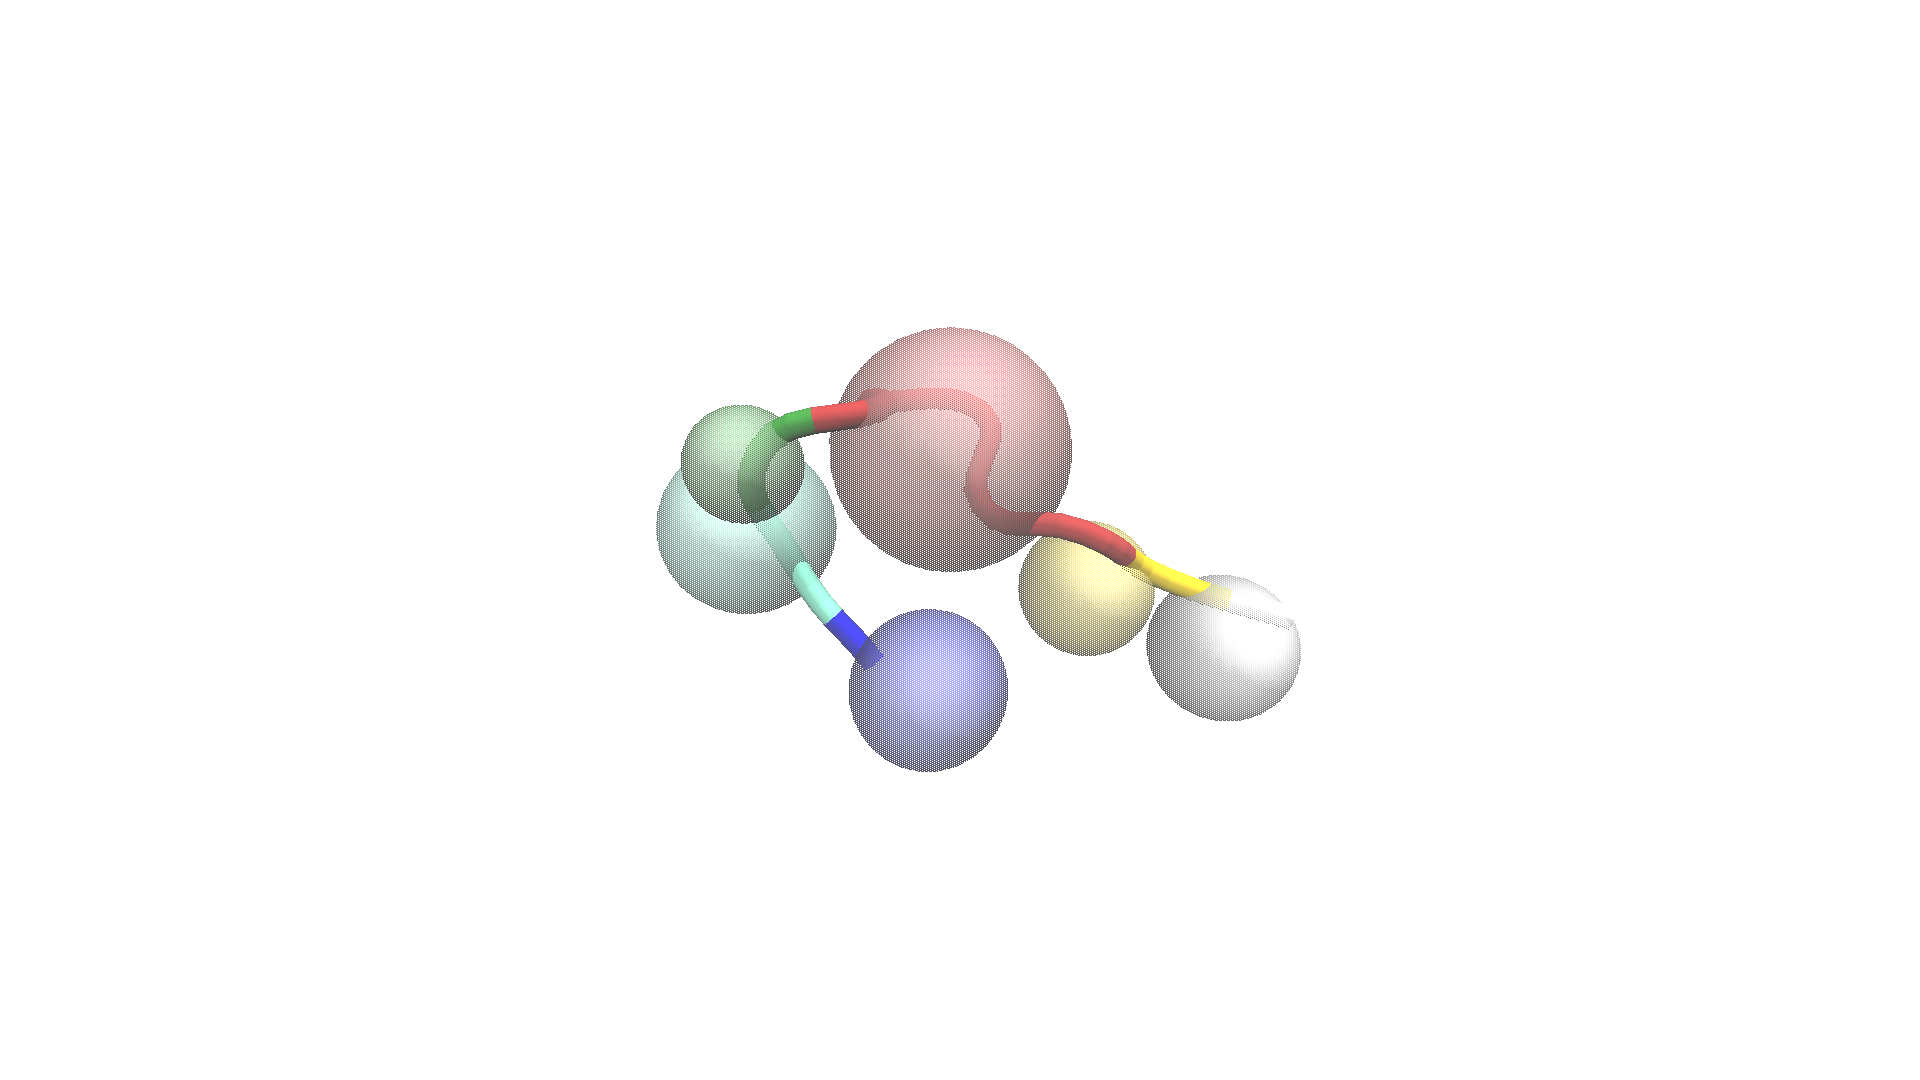
\includegraphics[width=0.25\textwidth, trim={22cm 6cm 22cm 6cm},clip]{CLN025_chignolin_beads.png}}
  \subfloat[Trp-cage]{
  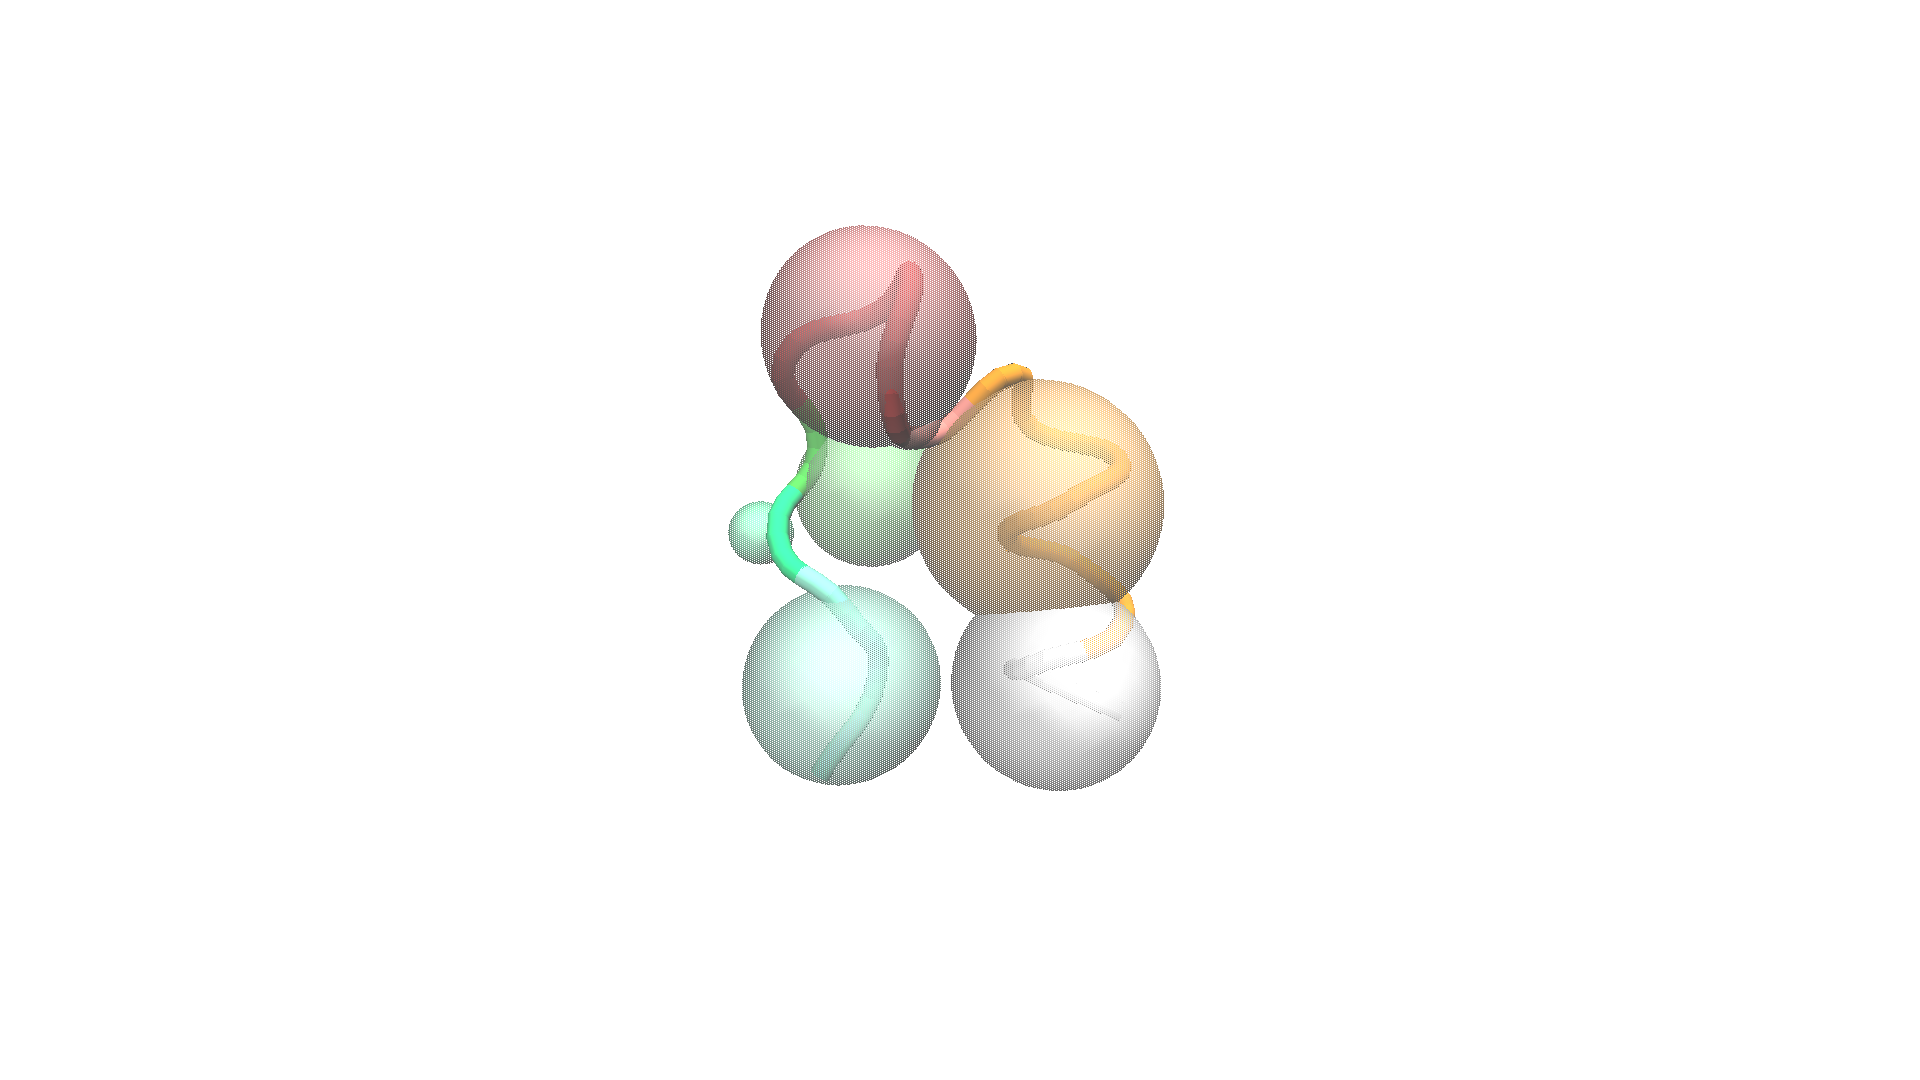
\includegraphics[width=0.25\textwidth, trim={22cm 6cm 22cm 6cm},clip]{2JOF_trp-cage_beads.png}}
  \subfloat[BBA]{
  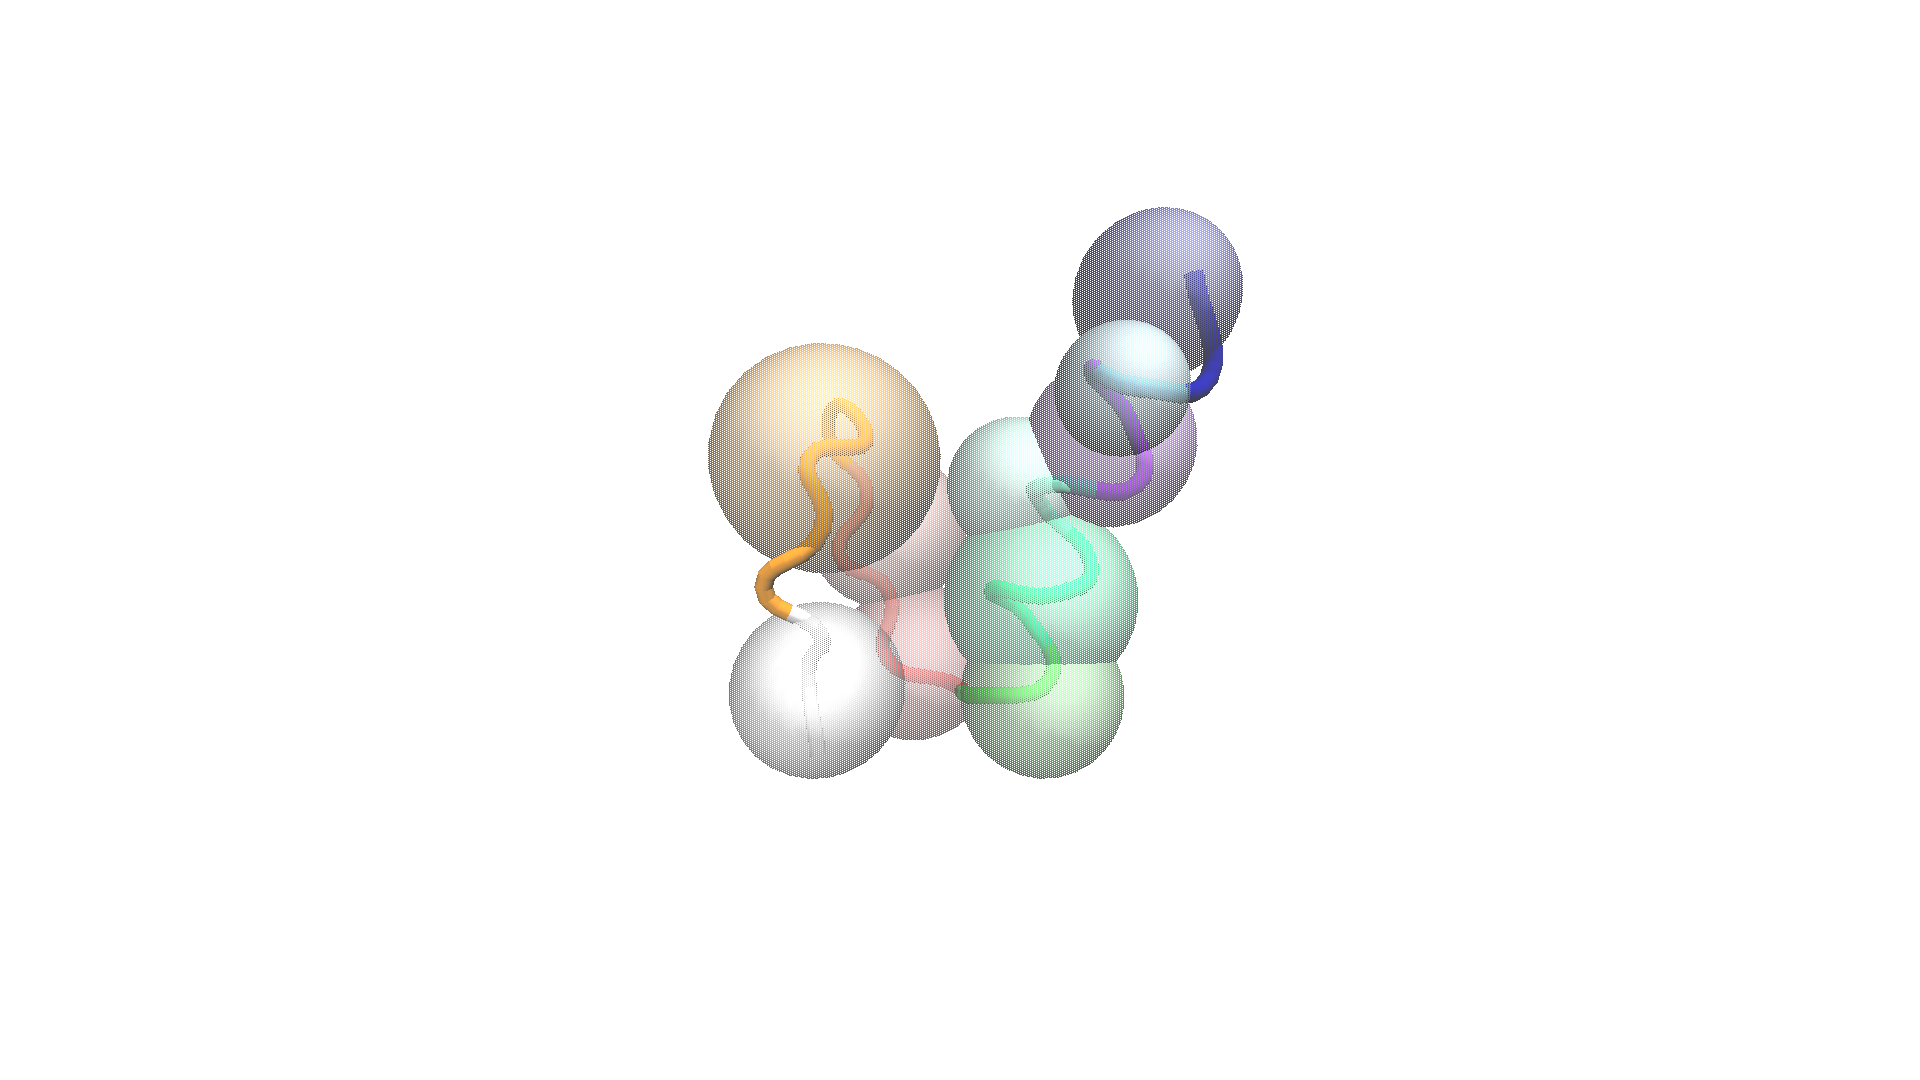
\includegraphics[width=0.25\textwidth, trim={22cm 6cm 22cm 6cm},clip]{1FME_BBA_beads.png}}
  \subfloat[Villin]{
  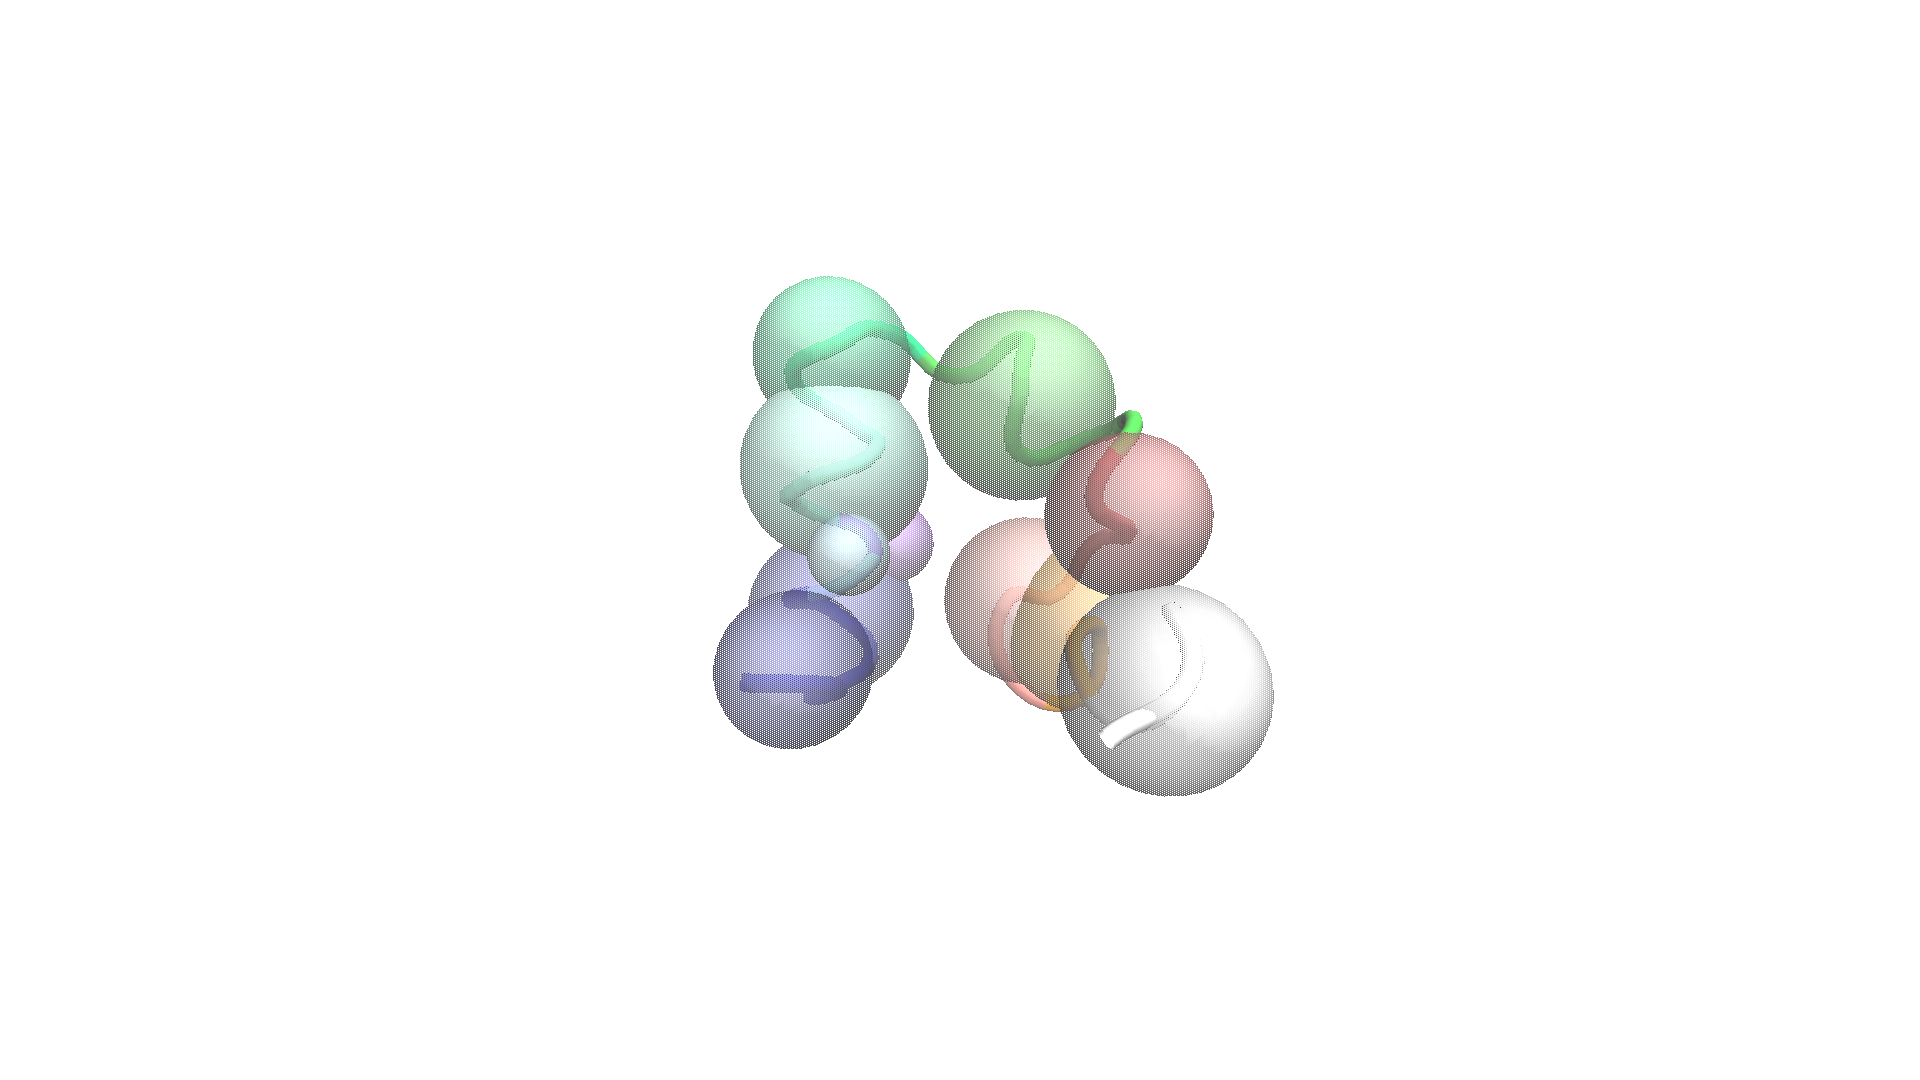
\includegraphics[width=0.25\textwidth, trim={22cm 6cm 22cm 6cm},clip]{2F4K_villin_beads.png}}\\
  \subfloat[BBL]{
  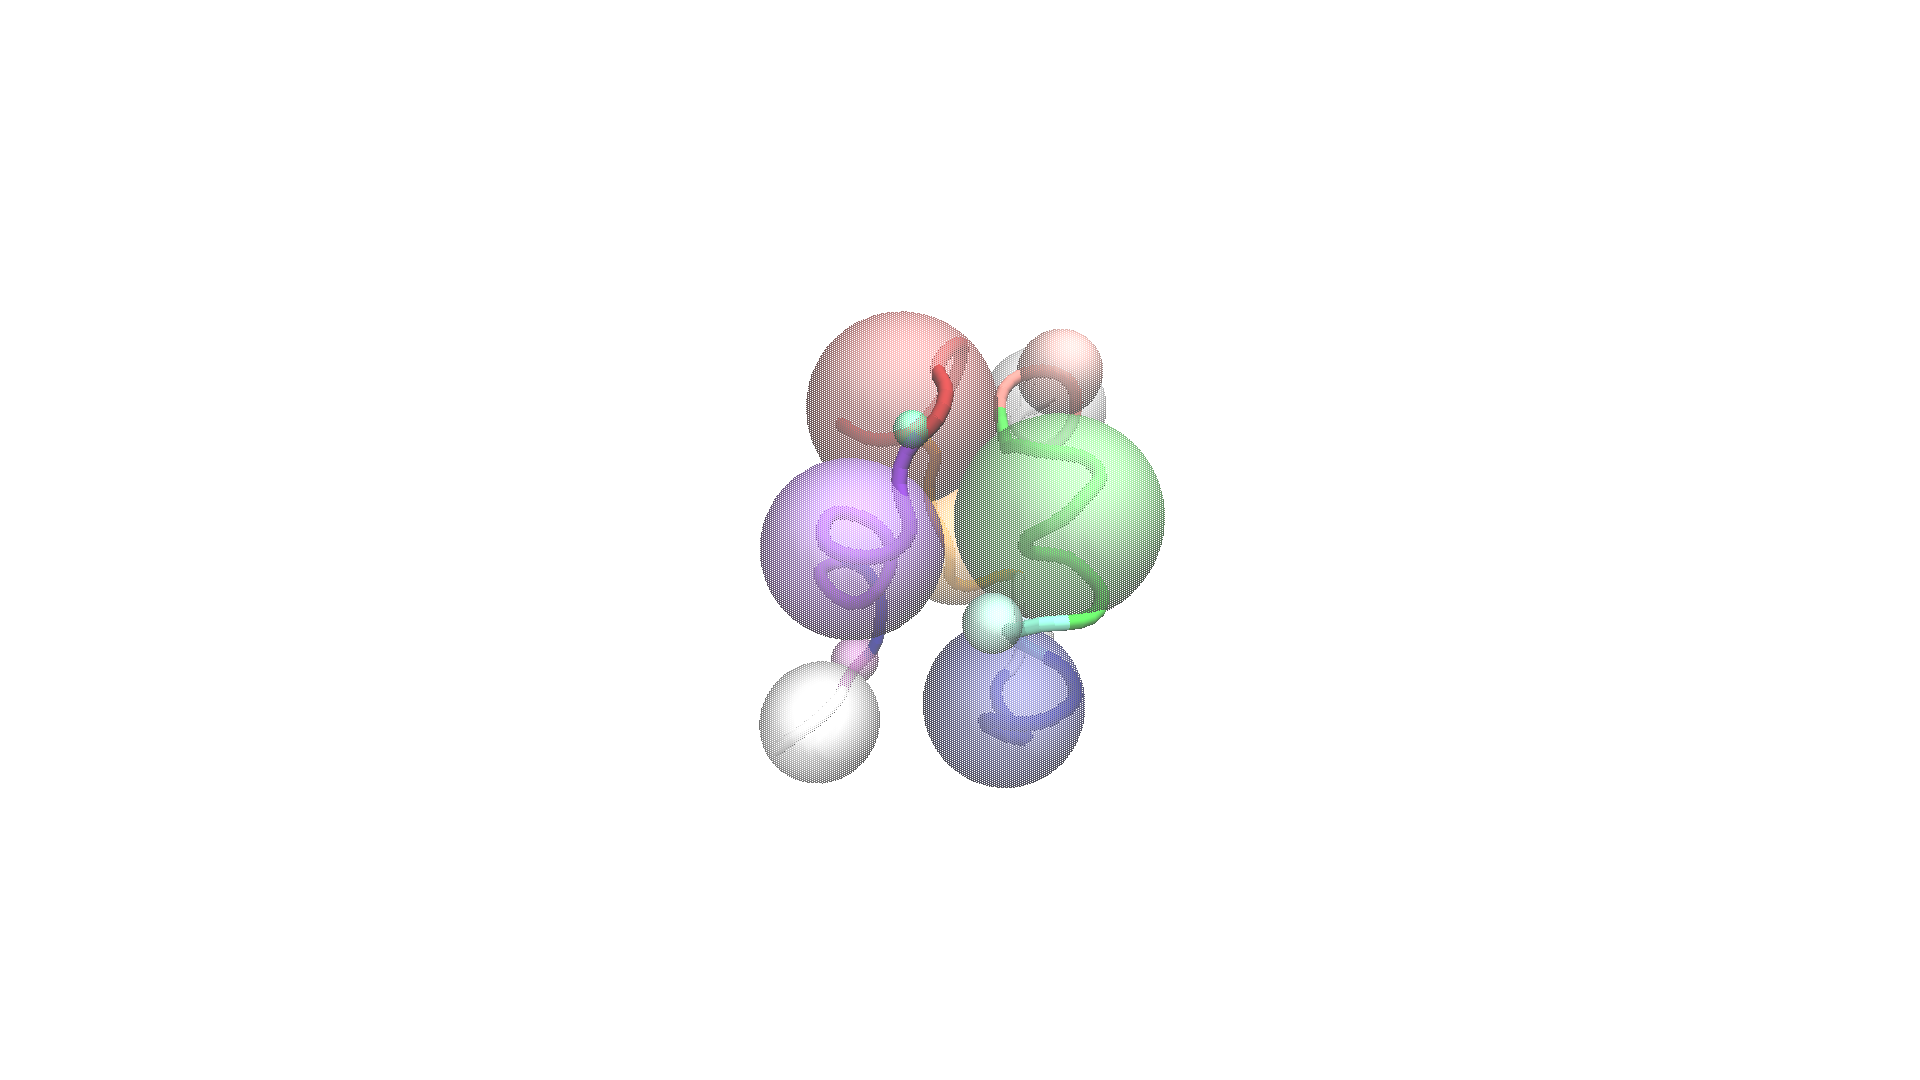
\includegraphics[width=0.25\textwidth, trim={22cm 6cm 22cm 6cm},clip]{2WAV_BBL_beads.png}}
  \subfloat[Protein B]{
  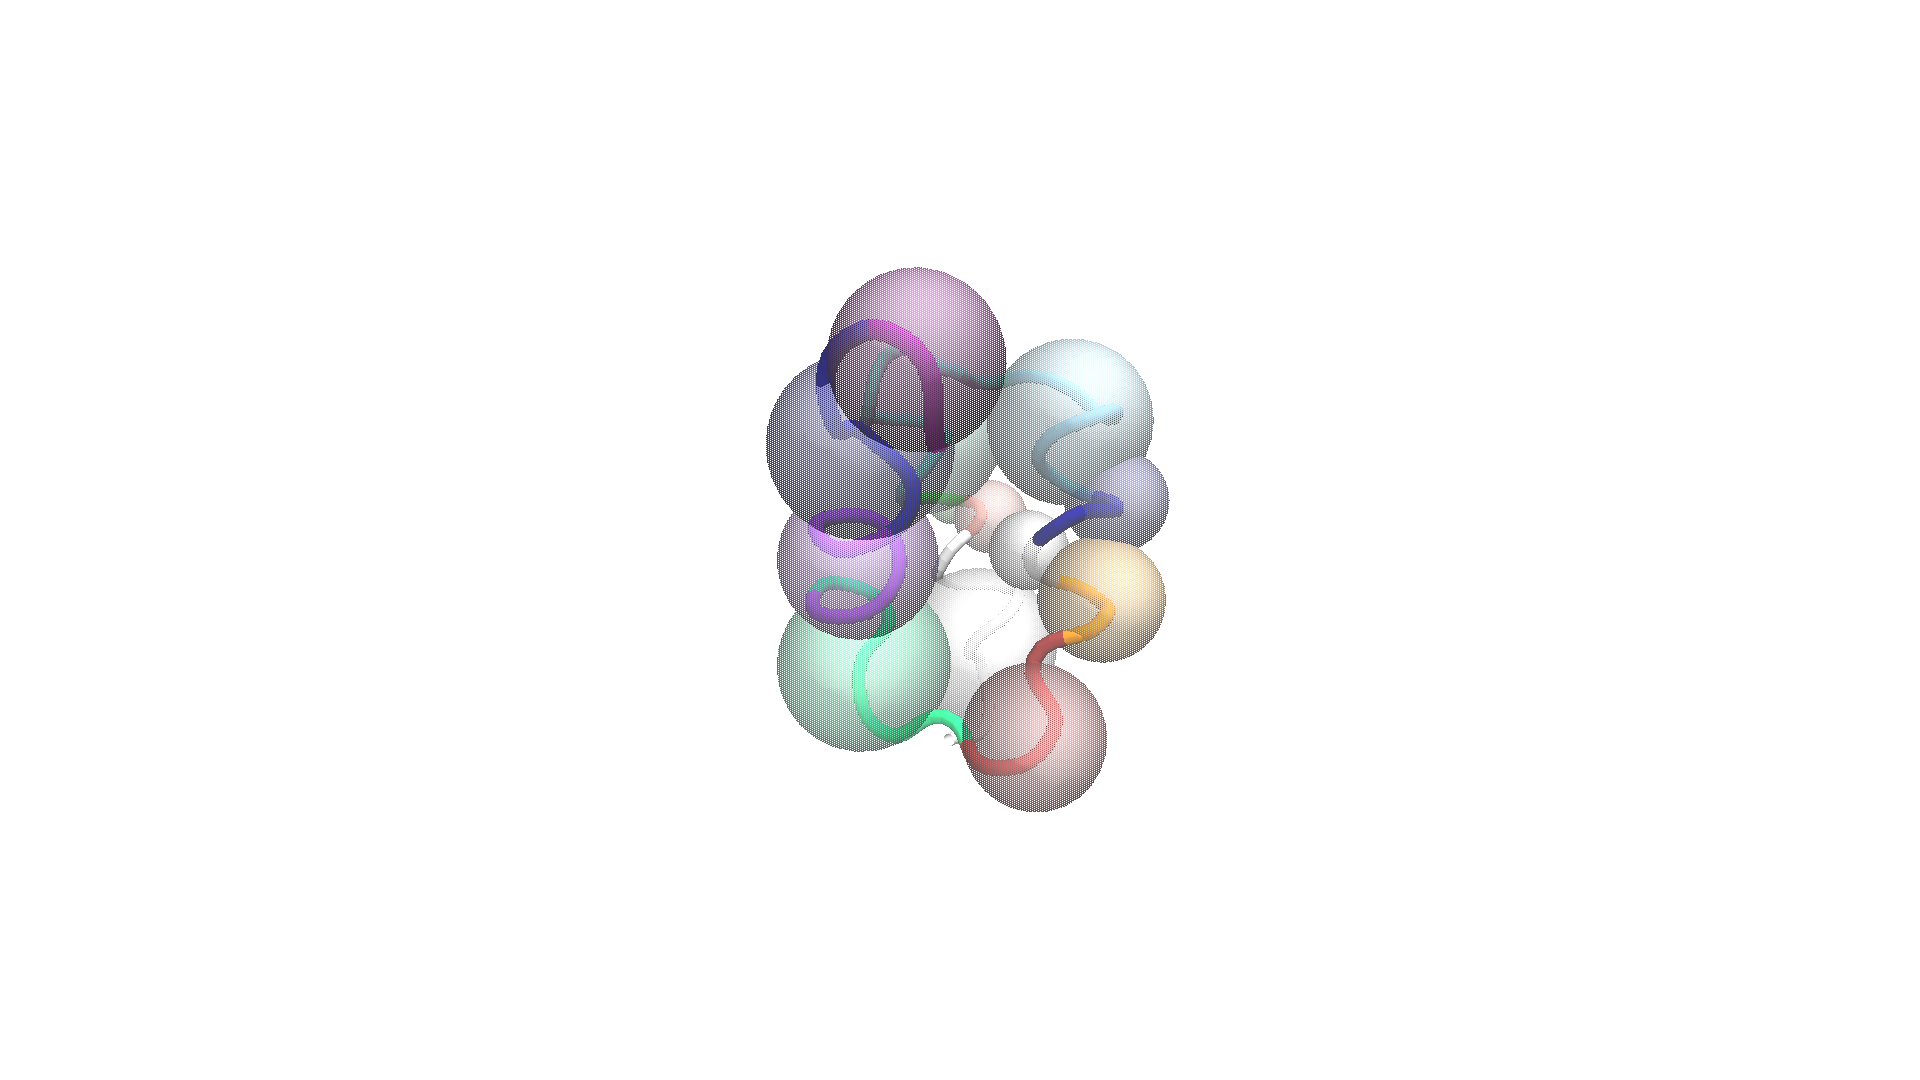
\includegraphics[width=0.25\textwidth, trim={22cm 6cm 22cm 6cm},clip]{PRB_protein_b_beads.png}}
  \subfloat[Homeodomain]{
  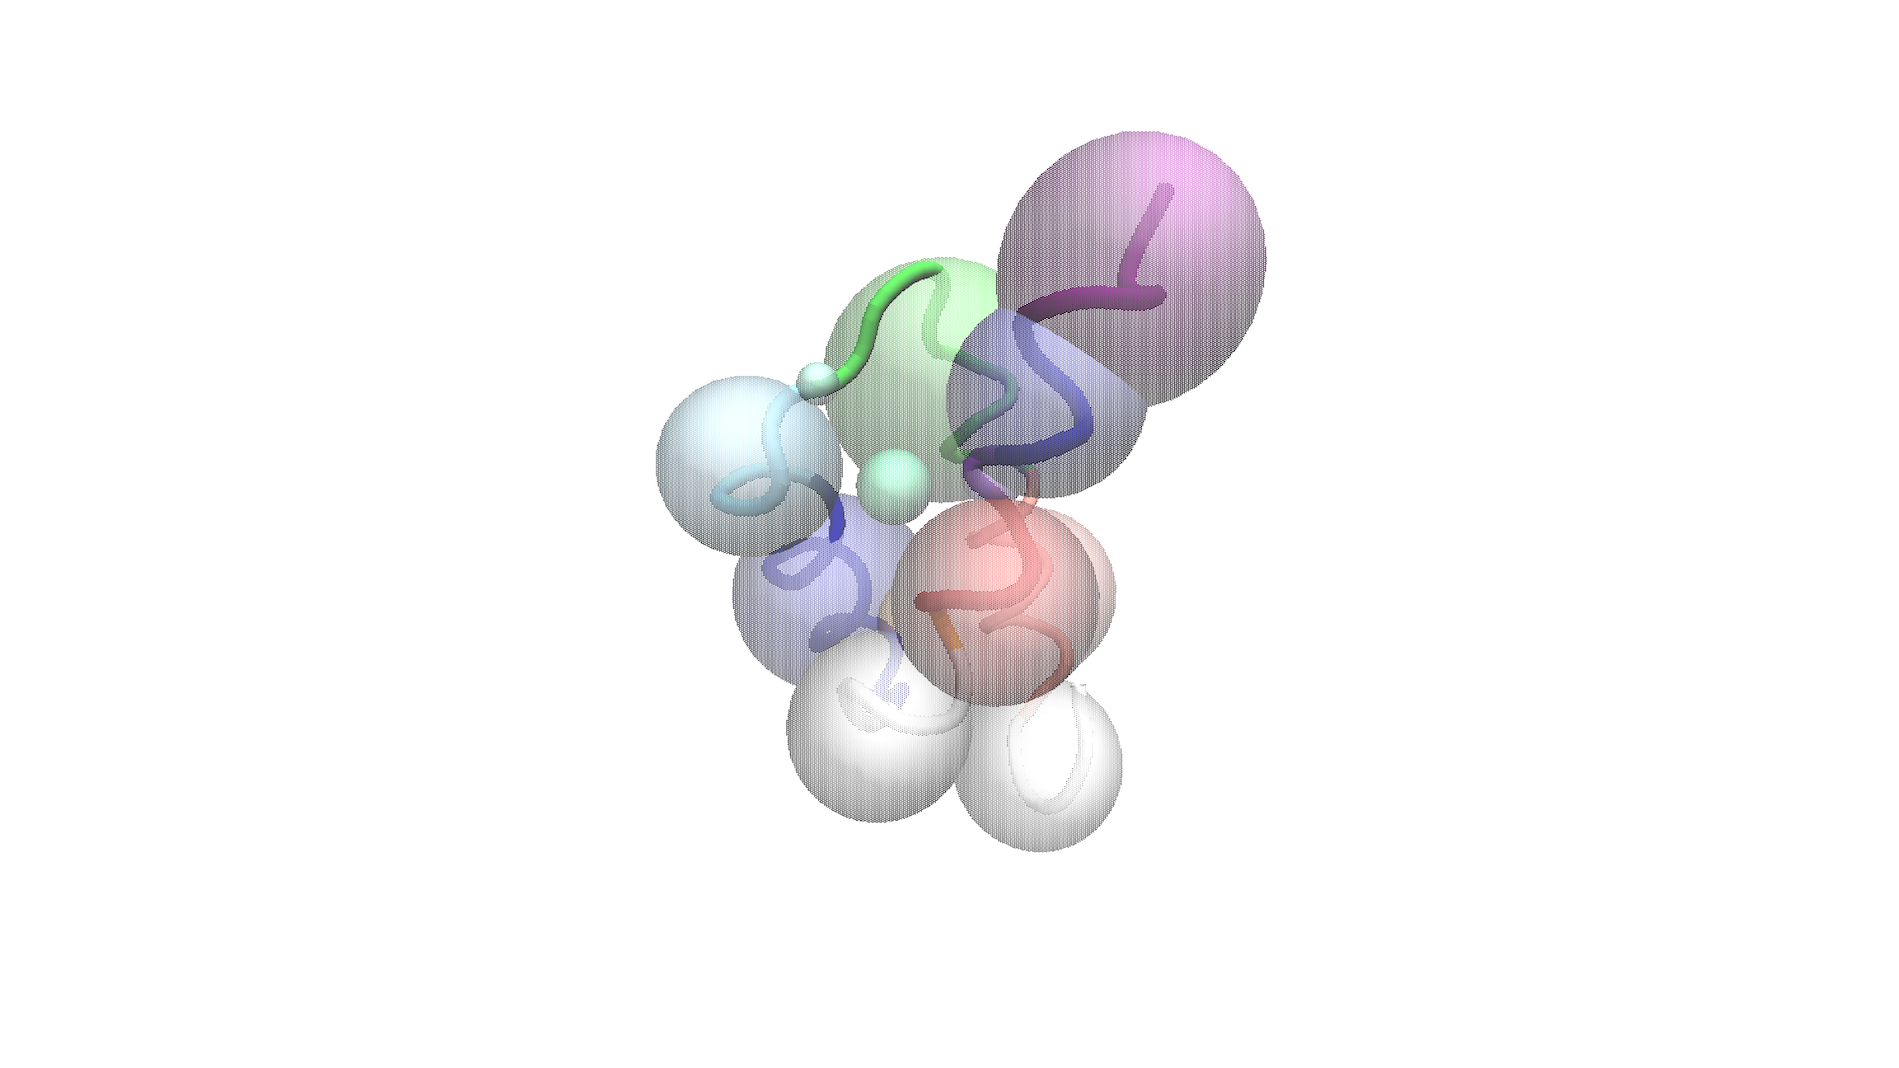
\includegraphics[width=0.25\textwidth, trim={18cm 3cm 18cm 3cm},clip]{UVF_homeodomain_beads.png}}
  \subfloat[Protein G]{
  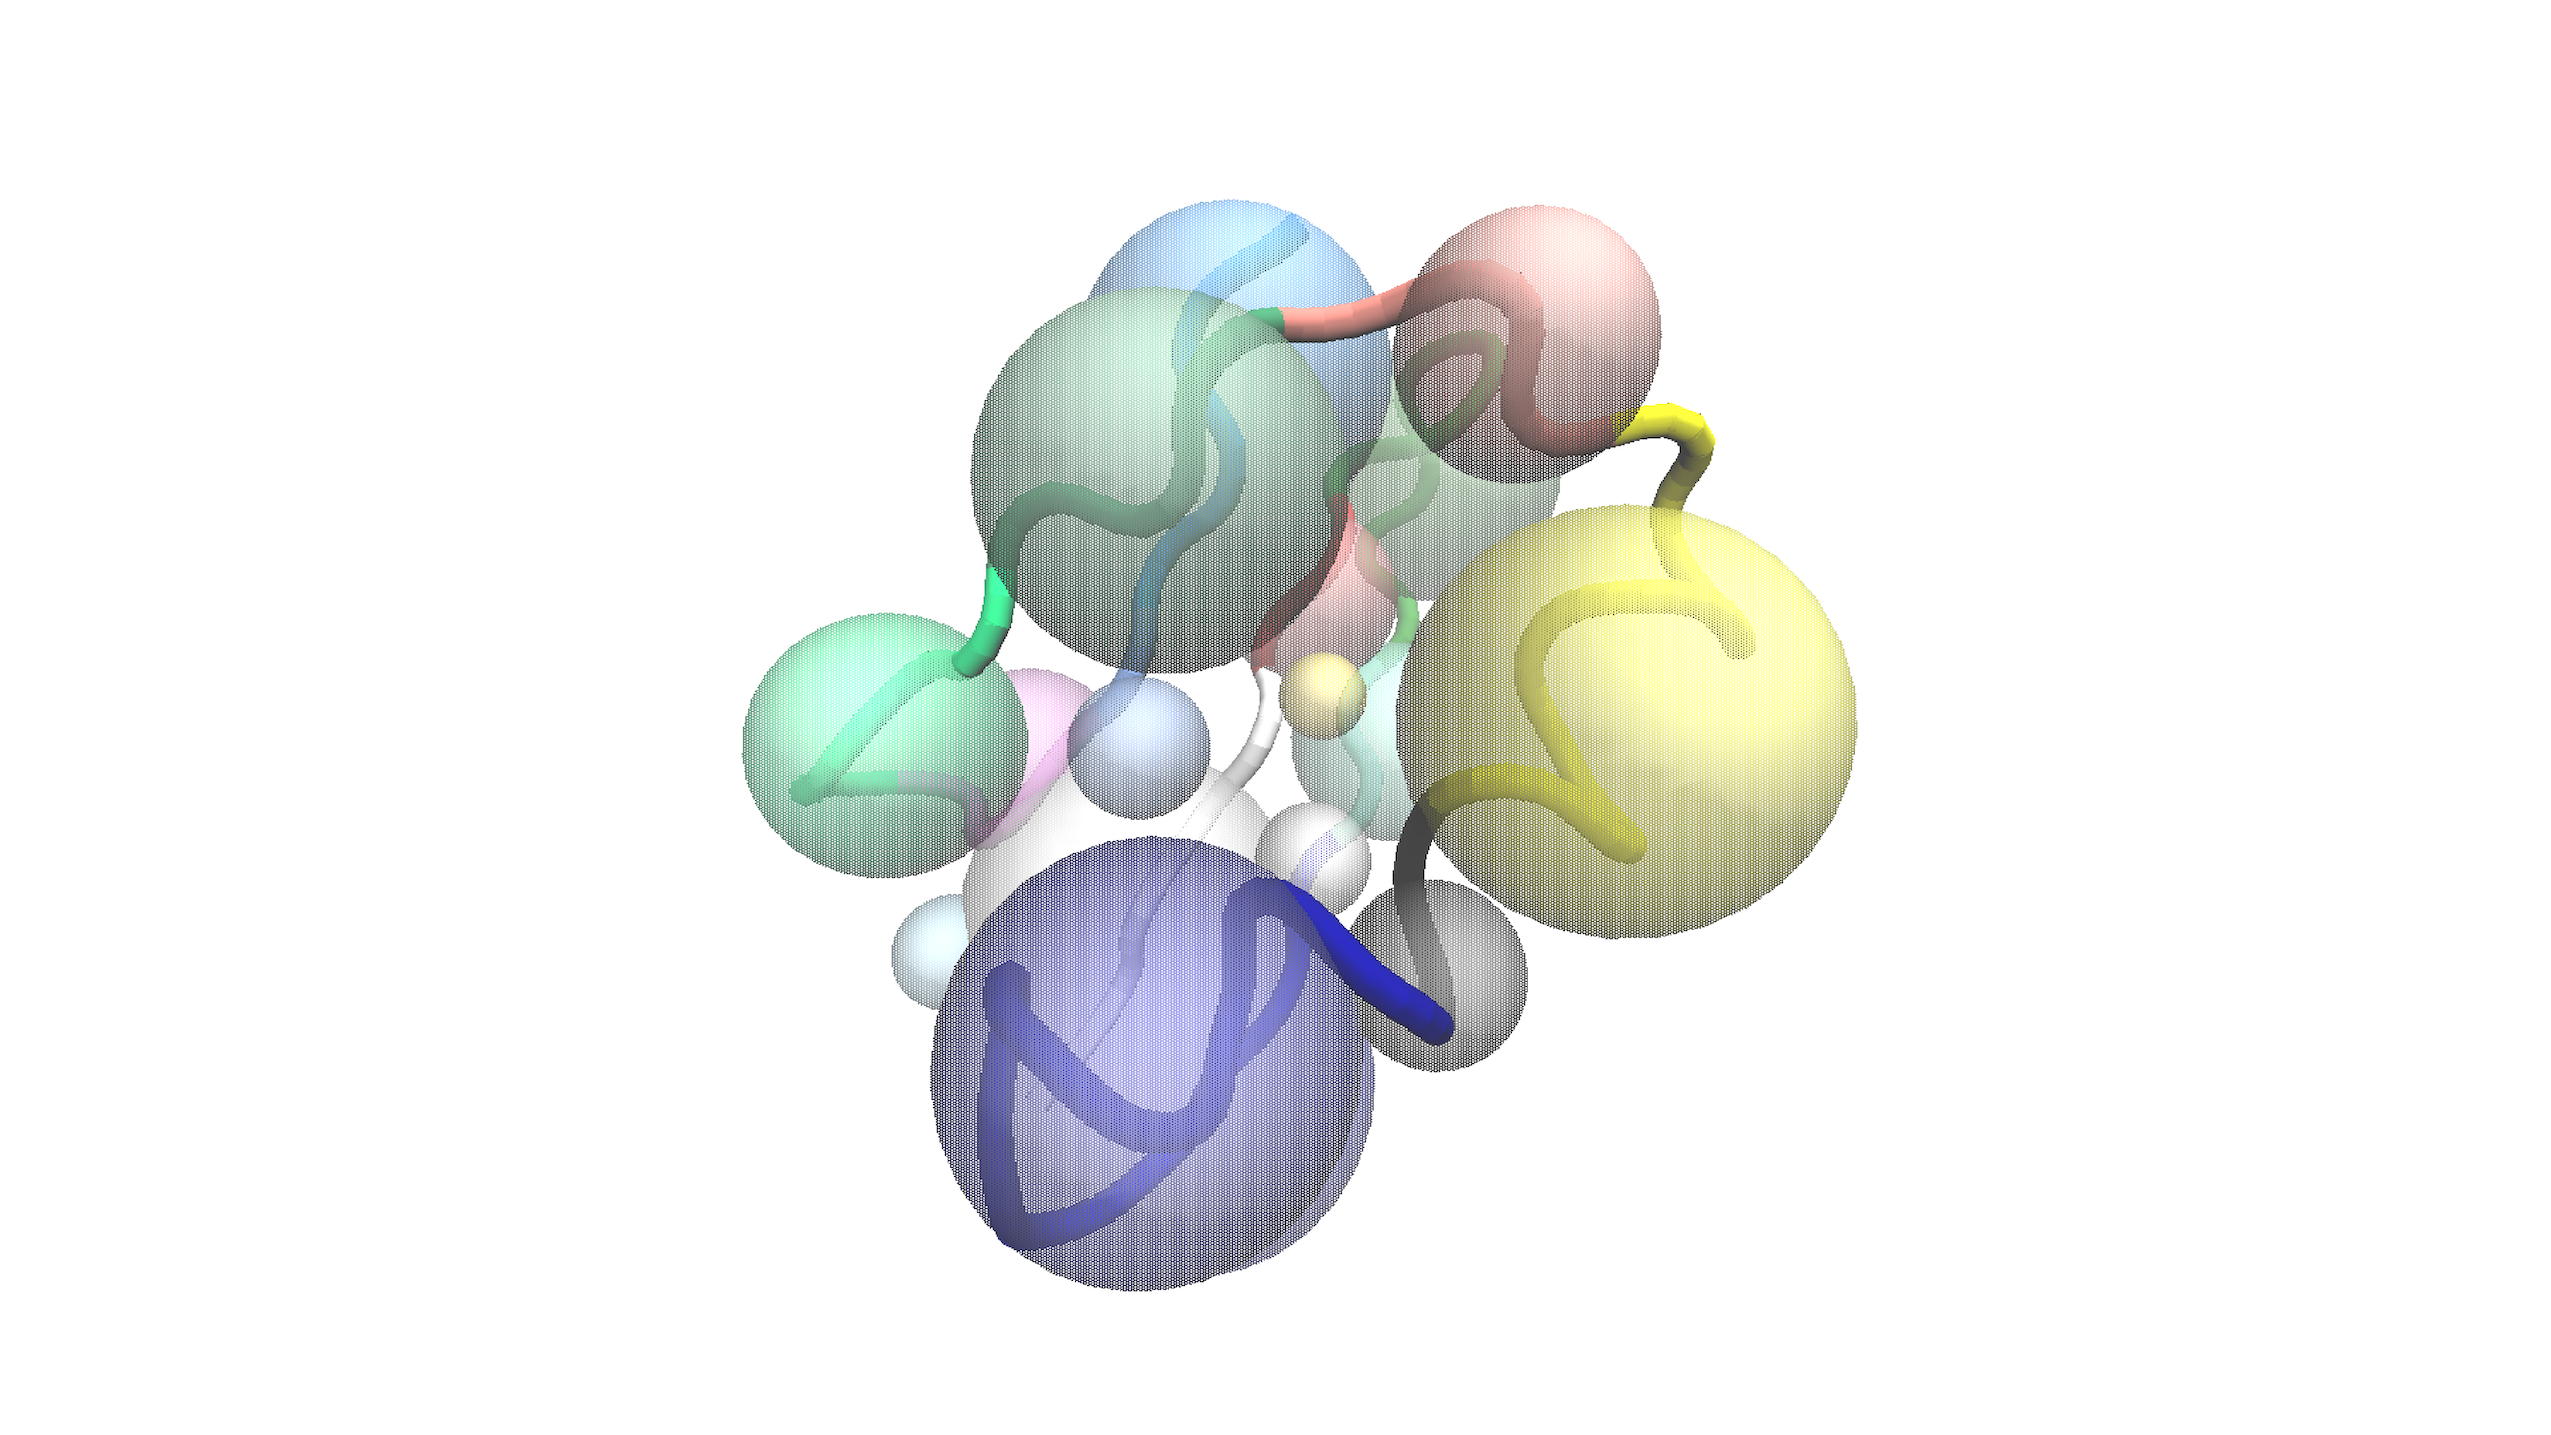
\includegraphics[width=0.25\textwidth, trim={18cm 3cm 18cm 3cm},clip]{NuG2_protein_g_all_beads_new.png}}\\
  \subfloat[$\alpha$3D]{
  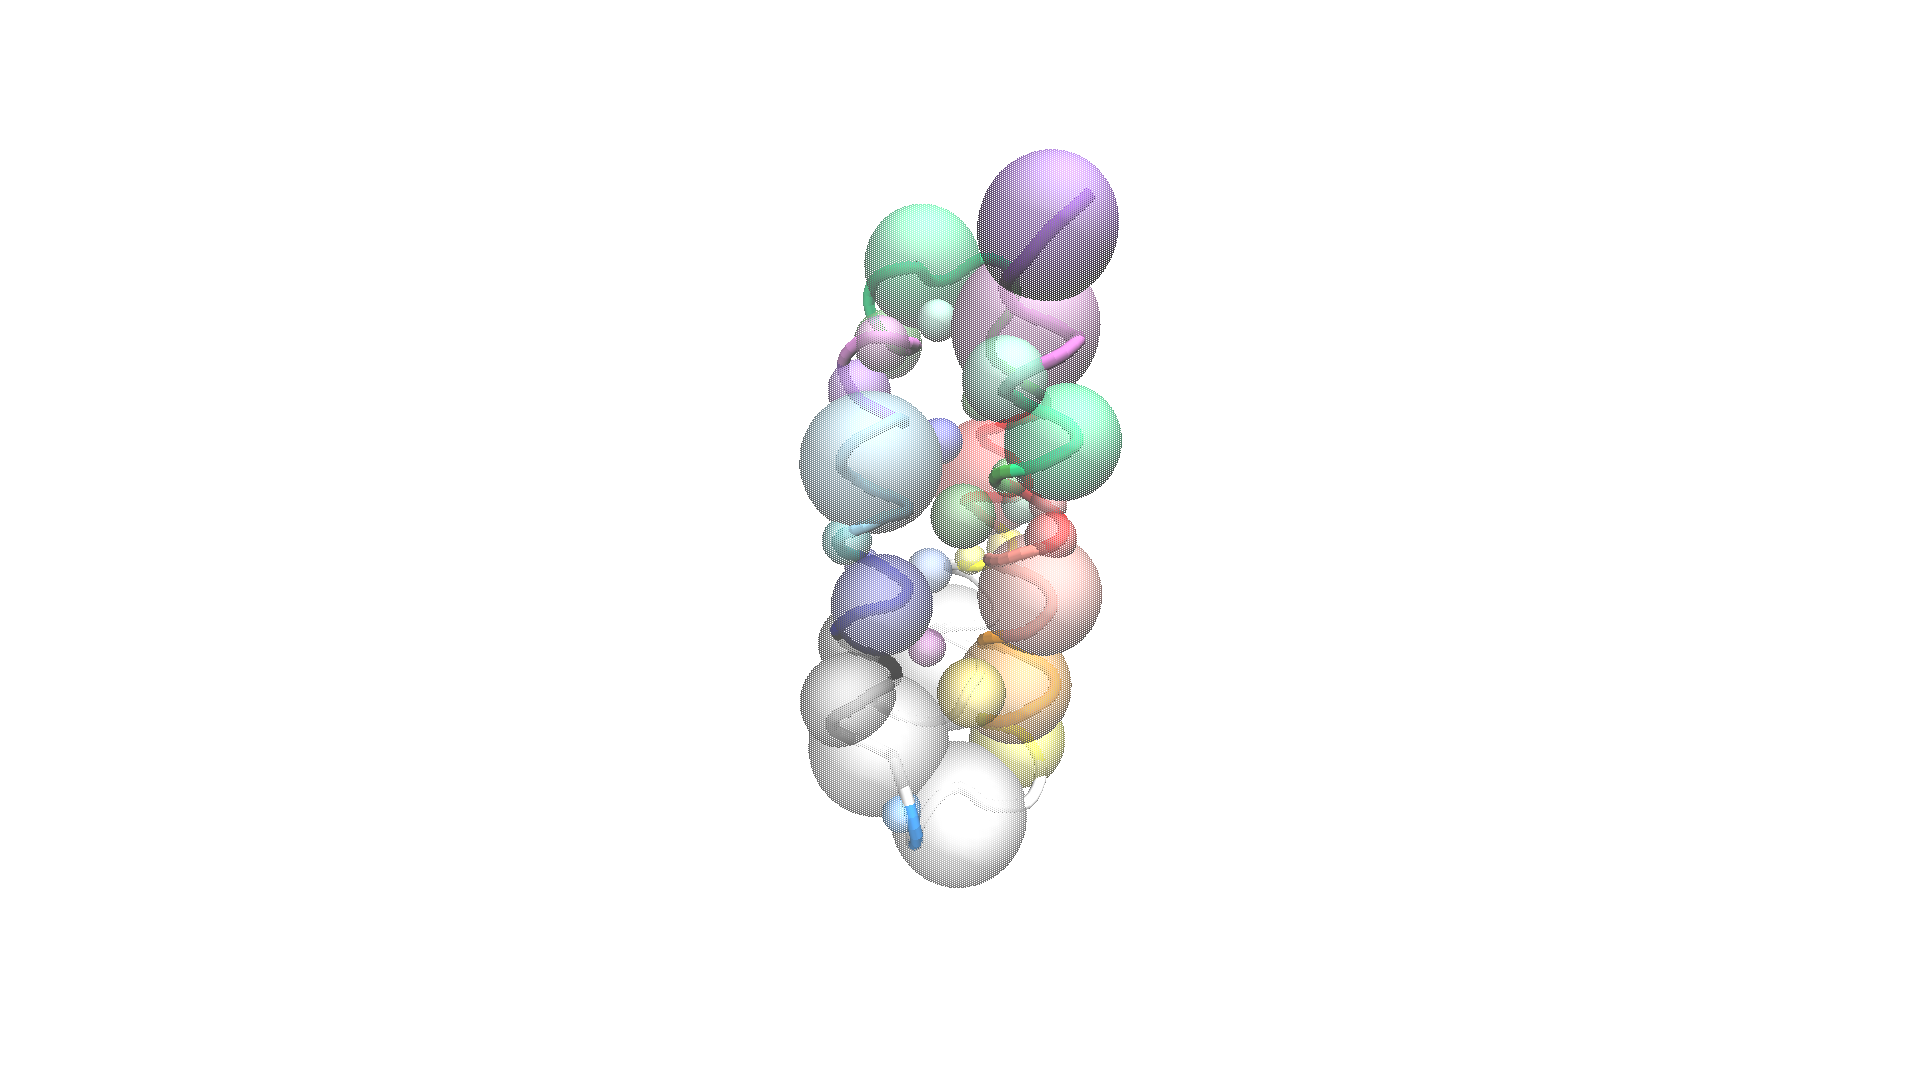
\includegraphics[width=0.25\textwidth, trim={22cm 6cm 22cm 3cm},clip]{A3D_alpha3D_beads.png}}
  \subfloat[$\lambda$-repressor]{
  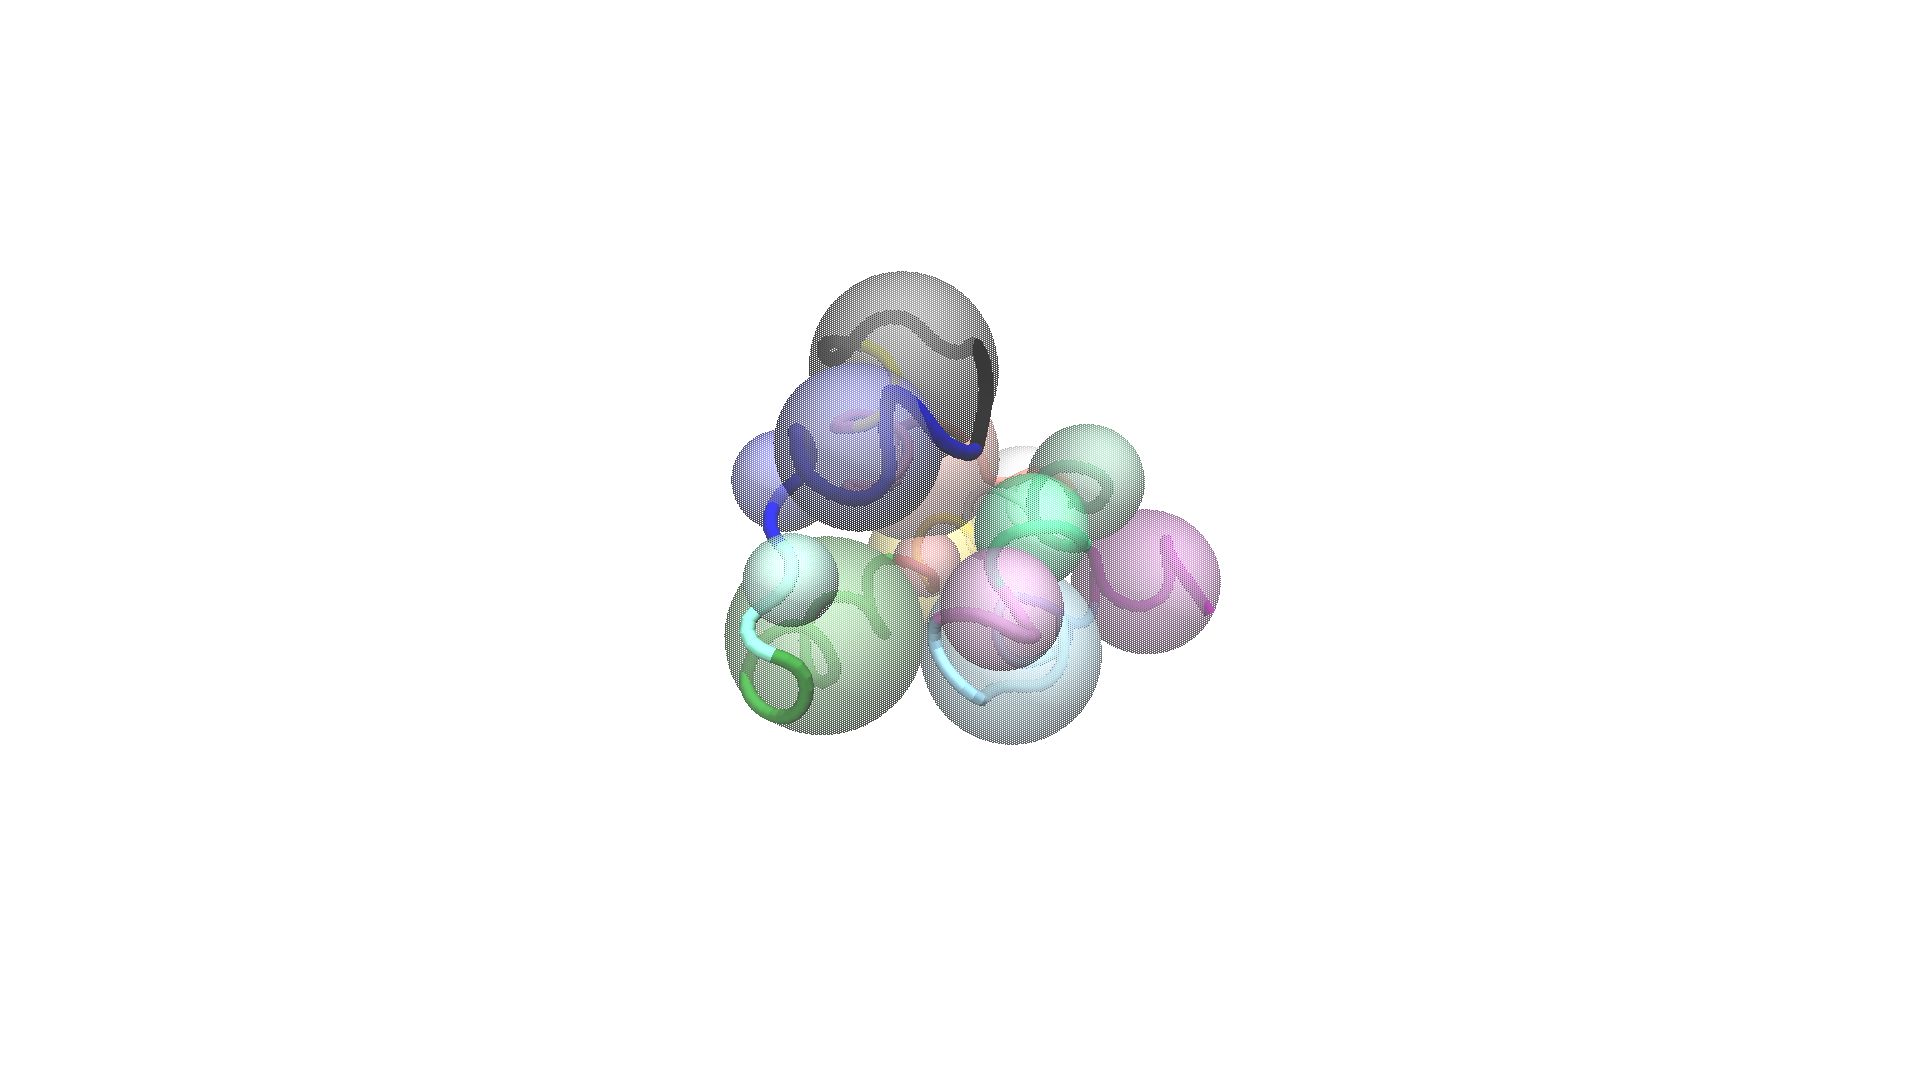
\includegraphics[width=0.25\textwidth, trim={22cm 6cm 22cm 6cm},clip]{lambda_repressor_beads.png}}
  \caption{\label{all_beads}The decomposition results of the 10 fast-folding proteins in the order of protein's size. The structures shown here are representatives selected from the folded metastable states we identified from the simulation data. And the different colors indicate the different assembly units. The transparent spheres over there are to give a concept that these units can be the candidates of a CG model. They are plotted with the center of masses of all heavy atoms within the unit and the radius of gyration of them.}
\end{figure}

\setlength{\parindent}{2em}

To check the consistency of the results from different proteins, we calculate the average size (number of heavy atoms) of the minimal assembly units for each protein. We plot the average size against the total heavy atom numbers of the corresponding protein. We also plot the data points of FIP35 and NTL9, the two proteins tested in the original paper of S3D\cite{Lrenzo_S3D}, so in fig-\ref{all_stat}, there are 12 data points in total. For most proteins, the average size of assembly units is between 20 to 30 heavy atoms, and there is a trend that larger proteins will also have larger assembly units. However, there are two proteins whose results are outside of this range: homeodomain's assembly units seem to be much larger than other proteins and $\alpha 3D$'s much smaller. This is because the dynamics of these two proteins are different from others, which we will discuss below.

\begin{figure}[htbp]
  \centering
  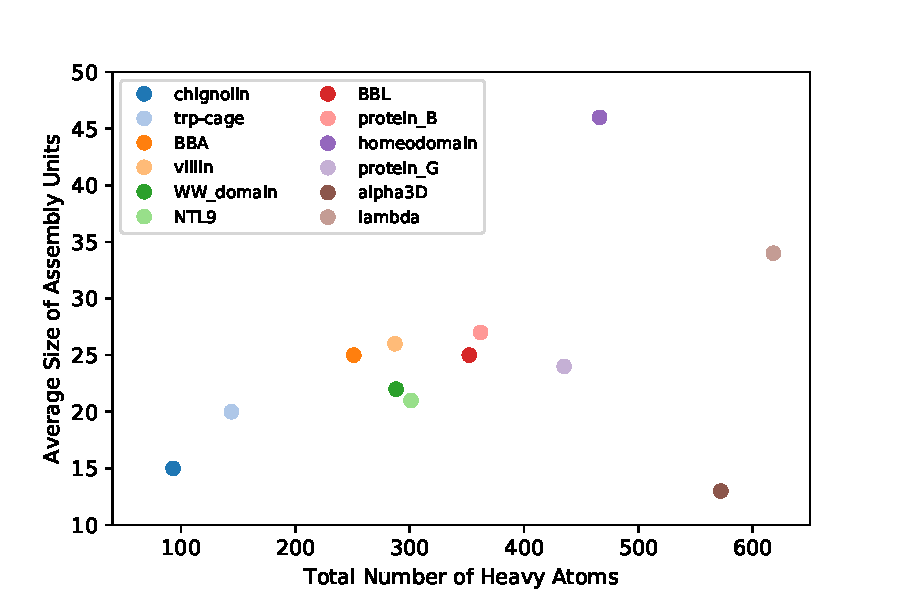
\includegraphics[width=1\textwidth]{stat_size_color.pdf}
  \caption{\label{all_stat}The average sizes of the assembly units against the sizes of all the proteins}
\end{figure}

\setlength{\parindent}{0em}

{\bf Homeodomain doesn't unfold very well.} We identified 3 metastable states for homeodomain, which are the unfolded, intermediate and folded state. In fig-\ref{UVF}, we show the contact maps of these 3 metastable states, which clearly indicates that in all of these 3 states the 3 cores of $\alpha$-helices are formed, {\it i.e.} the folding process of homeodomain mainly happens on the tertiary structure. This is not surprising, because the data we use is not from a natural homeodomain, but a designed mutant, UVF, whose stability has been greatly strengthened\cite{UVF_origin}.The stability of UVF's secondary structure caused 2 results: 1) its conformation is always very compact, which leads to a small number of coherent domains for each metastable state; 2) the relatively high structural similarity of these 3 states' conformations makes their coherent domains more similar, {\it i.e.} there are many common boundary points of coherent domains from different states. As a consequence of these 2 factors, it is reasonable that we obtained less and larger minimal assembly units.

\begin{figure}[htbp]
  \centering
  \subfloat[Unfolded State]{
  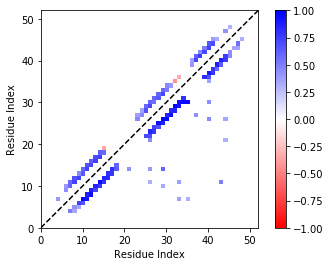
\includegraphics[width=0.33\textwidth]{UVF_contact_HMM_3_state_2_10TICA.png}}
  \subfloat[Intermediate State]{
  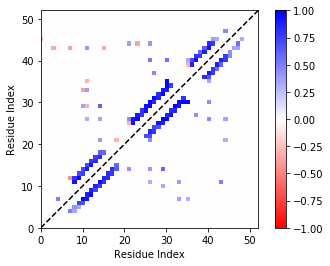
\includegraphics[width=0.33\textwidth]{UVF_contact_HMM_3_state_0_10TICA.png}}
  \subfloat[Folded State]{
  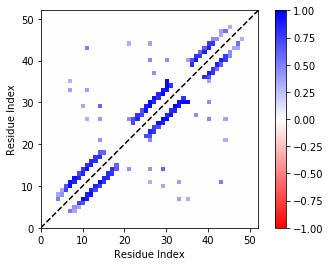
\includegraphics[width=0.33\textwidth]{UVF_contact_HMM_3_state_1_10TICA.png}}
  \caption{\label{UVF}The contact maps of the 3 metastable states of homeodomain (above diagonal) against the folded state (below diagonal). Blue indicates native contacts and red the non-native ones. Cutoff distance for contact formation is 0.4 nm. Only contacts formed in over $30\%$ frames are shown.}
\end{figure}

\setlength{\parindent}{0em}

{\bf The dynamics of $\alpha 3D$ is more frustrated.} $\alpha 3D$ is a {\it de novo} designed protein\cite{A3D_de_novo}. Though its folding process is very fast \cite{A3D_fast_folder}, the dynamics is relatively frustrated. R. B. Best, et al. have demonstrated that the native contacts are not remarkably preferred during the folding process\cite{frustration} by using 1) a log-ratio of lifetimes of contacts on transition paths (TP) and unfolded state; and 2) a Bayesian measure of how predictive the formation of each contact is for being on a TP. Specifically, it was demonstrated that not like other natural proteins, nonnative contacts also play an important role in the folding mechanism determination of $\alpha 3D$\cite{A3D_frustration}.

\setlength{\parindent}{2em}

In addition, we also found that for $\alpha 3D$, there are 2 metastable states which are well-folded with a difference in the second loop region as shown in fig-\ref{A3D_contact}, where the contacts are highly frustrated\cite{Justin_frustration}. While we haven't observed a similar multiple folded state phenomenon on other proteins. Both of these results show that the dynamics of $\alpha 3D$ is more frustrated than other proteins, therefore, different regions of the molecule are less dynamically correlated. As a result, we need more and smaller assembly units (a finer mapping) to capture its long-timescale dynamics. 

\begin{figure}[htbp]
  \centering
  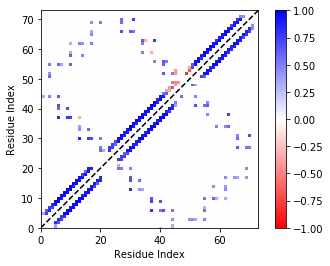
\includegraphics[width=0.5\textwidth]{A3D_contact_HMM_5_state_4_contacts.png}
  \caption{\label{A3D_contact}The contact maps of the 2 folded metastable states of $\alpha 3D$. Since the state shown in the below diagonal has the same structure in the second loop as the structure measured (PDB ID: 2A3D), we chose it as the native state. Blue indicates native contacts and red the non-native ones. Cutoff distance for contact formation is 0.4 nm. Only contacts formed in over $30\%$ frames are shown.}
\end{figure}

\setlength{\parindent}{0em}

{\bf A Modified Version of S3D for IDPs} Besides fast-folding proteins, we also applied S3D on 2 intrinsically disordered proteins. We found that S3D could not be directly applied on IDPs. Modification is needed extend application to IDPs. The issue is caused by the dynamics of IDPs, which is different from folded proteins. Since IDPs are very flexible and don't have specific folded structures\cite{IDP}, we cannot identify the metastable states as we did before\cite{IDP_dynamics}. However, because IDPs' dynamical characteristics will change under different conditions (such as different denaturant concentrations), we think that it makes sense to use space time diffusion map to perform decomposition on the data under different conditions, then combine these results to obtain the assembly units as their intersection. To accomplish this, we replace the metastable states with trajectories from different simulations.

\setlength{\parindent}{2em}

We applied this modified S3D on 2 IDPs, ACTR and MYC. The simulation data we use contains 6 $2\mu s$-long trajectories of ACTR under different urea concentrations\cite{ACTR} and 4 trajectories of MYC with length vary between $2-3\mu s$ under different NaCl concentrations\cite{MYC}. The minimal assembly units of these 2 IDPs are shown in fig-\ref{IDP_all_beads}. 

\begin{figure}[htbp]
  \centering
  \subfloat[ACTR]{
  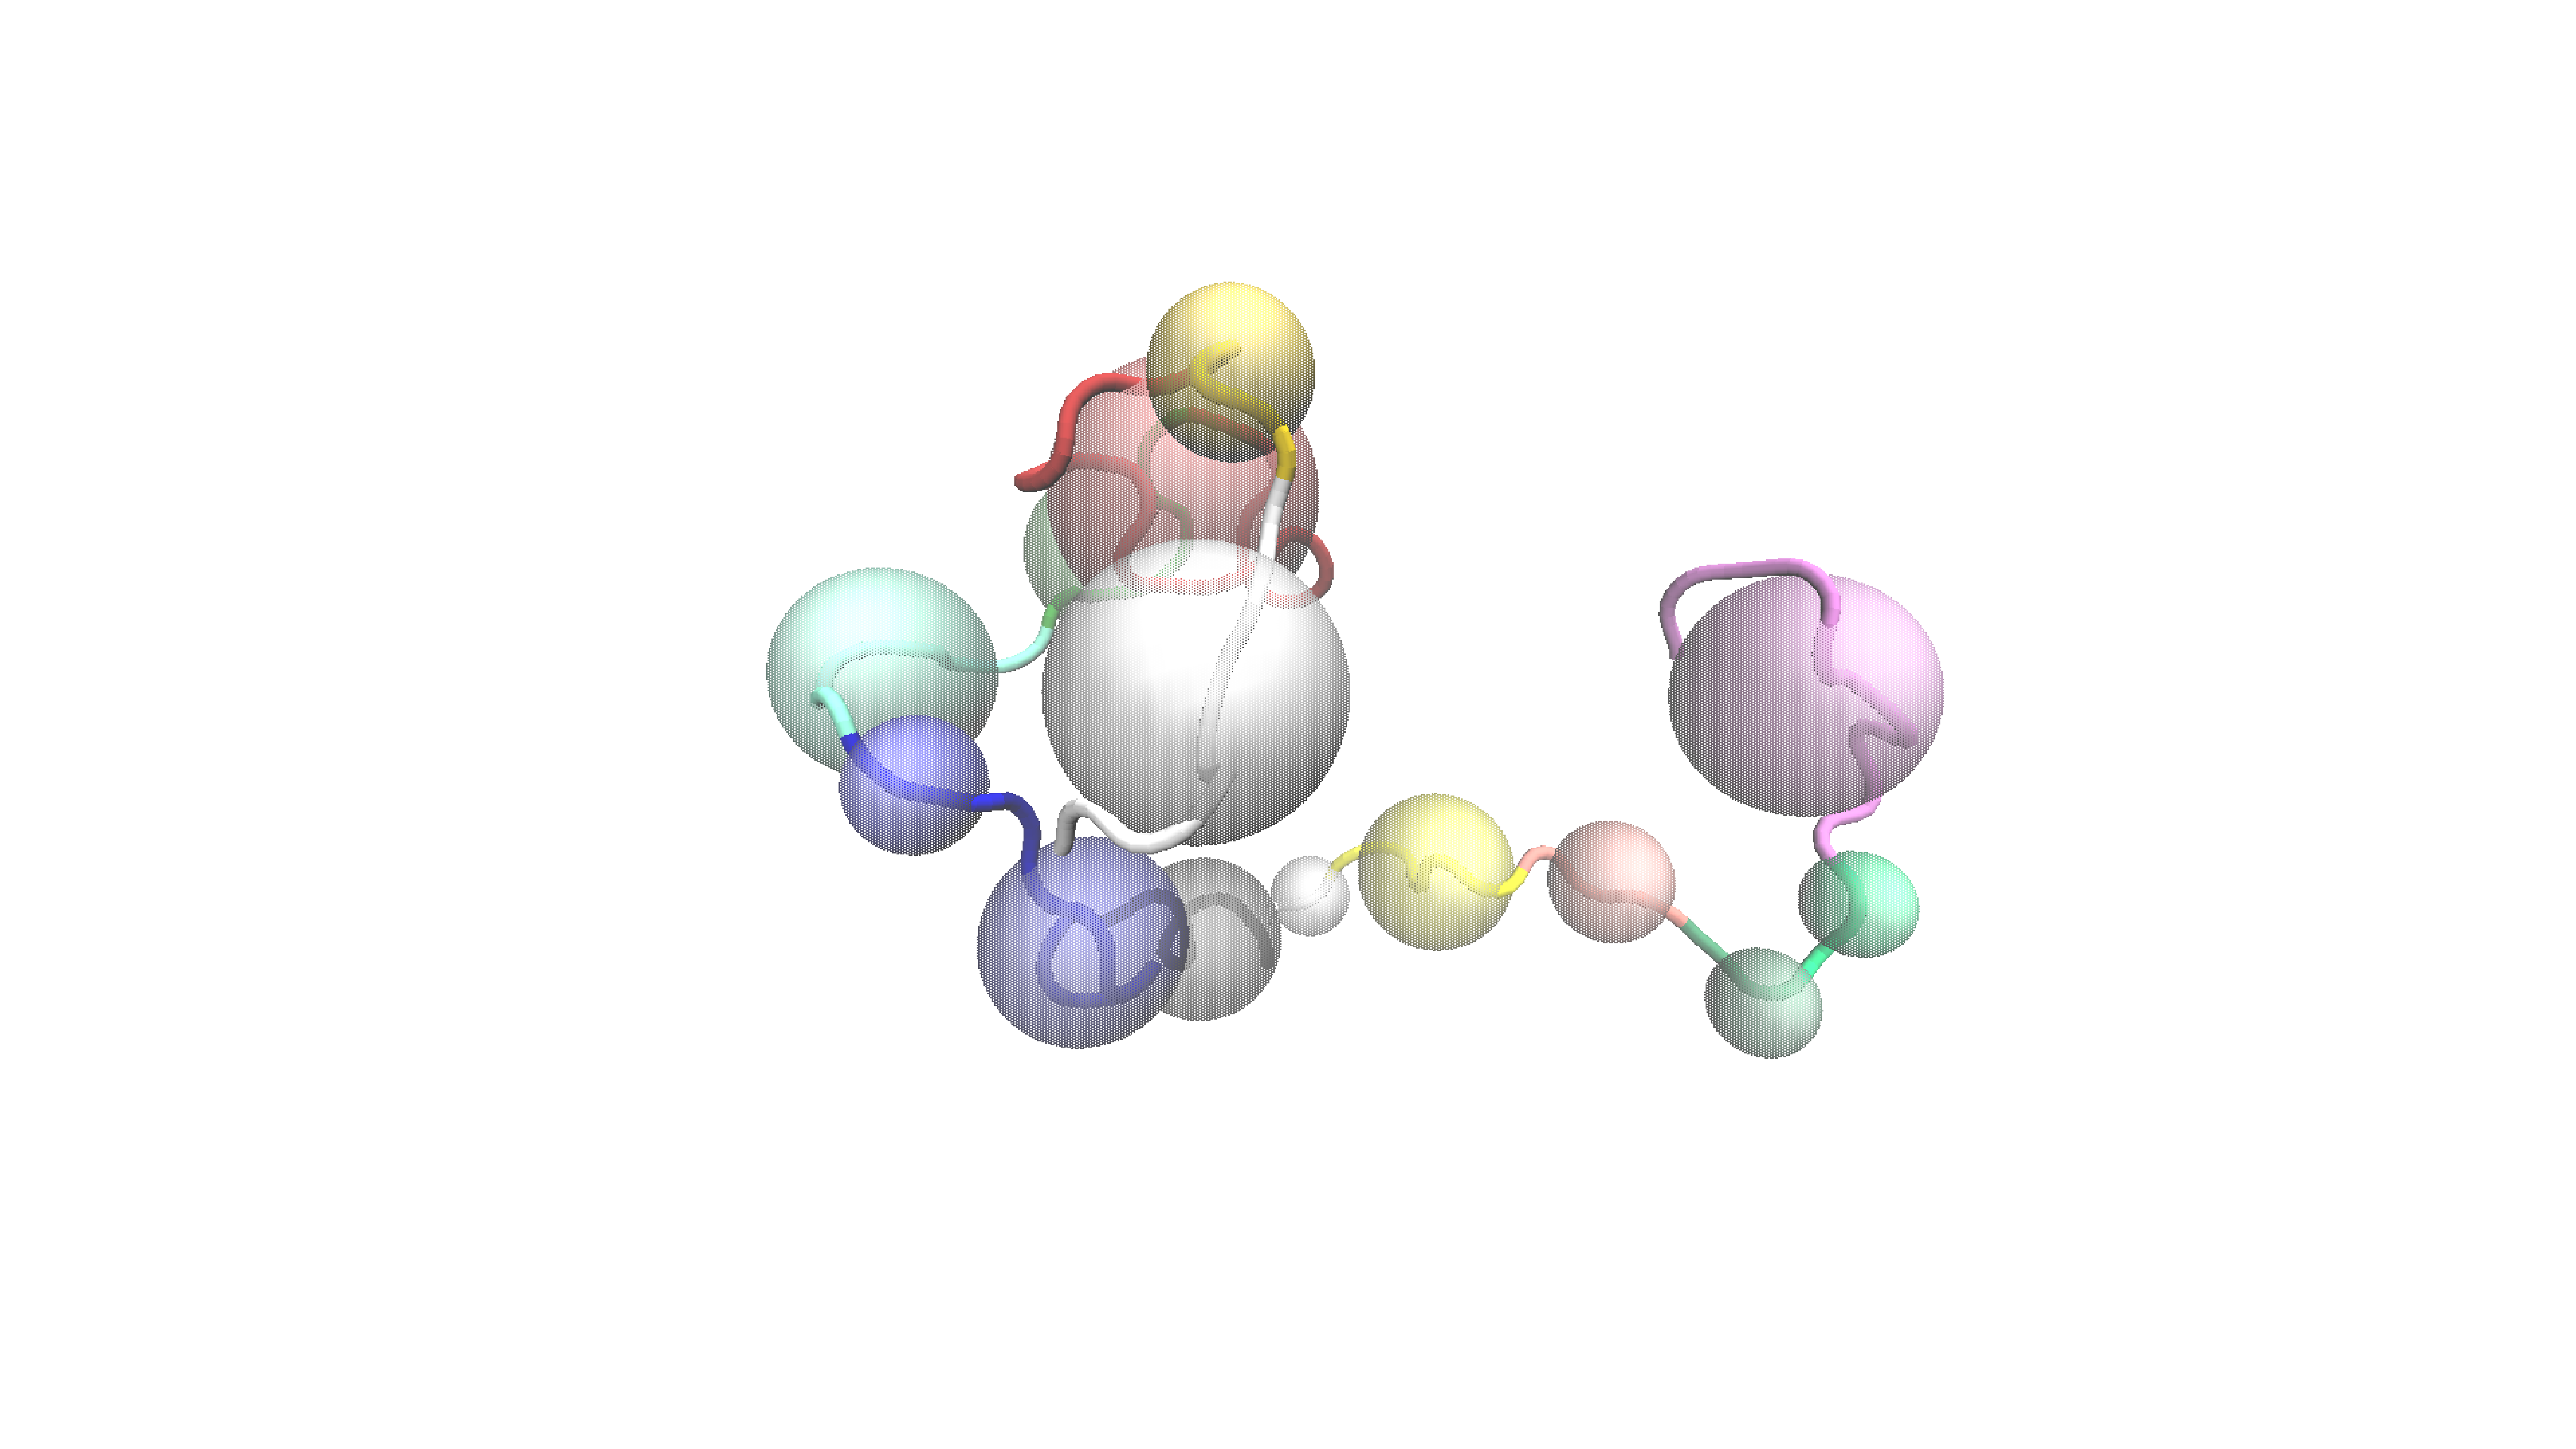
\includegraphics[width=0.5\textwidth, trim={35cm 18cm 35cm 18cm},clip]{ACTR_all_beads.png}}
  \subfloat[MYC]{
  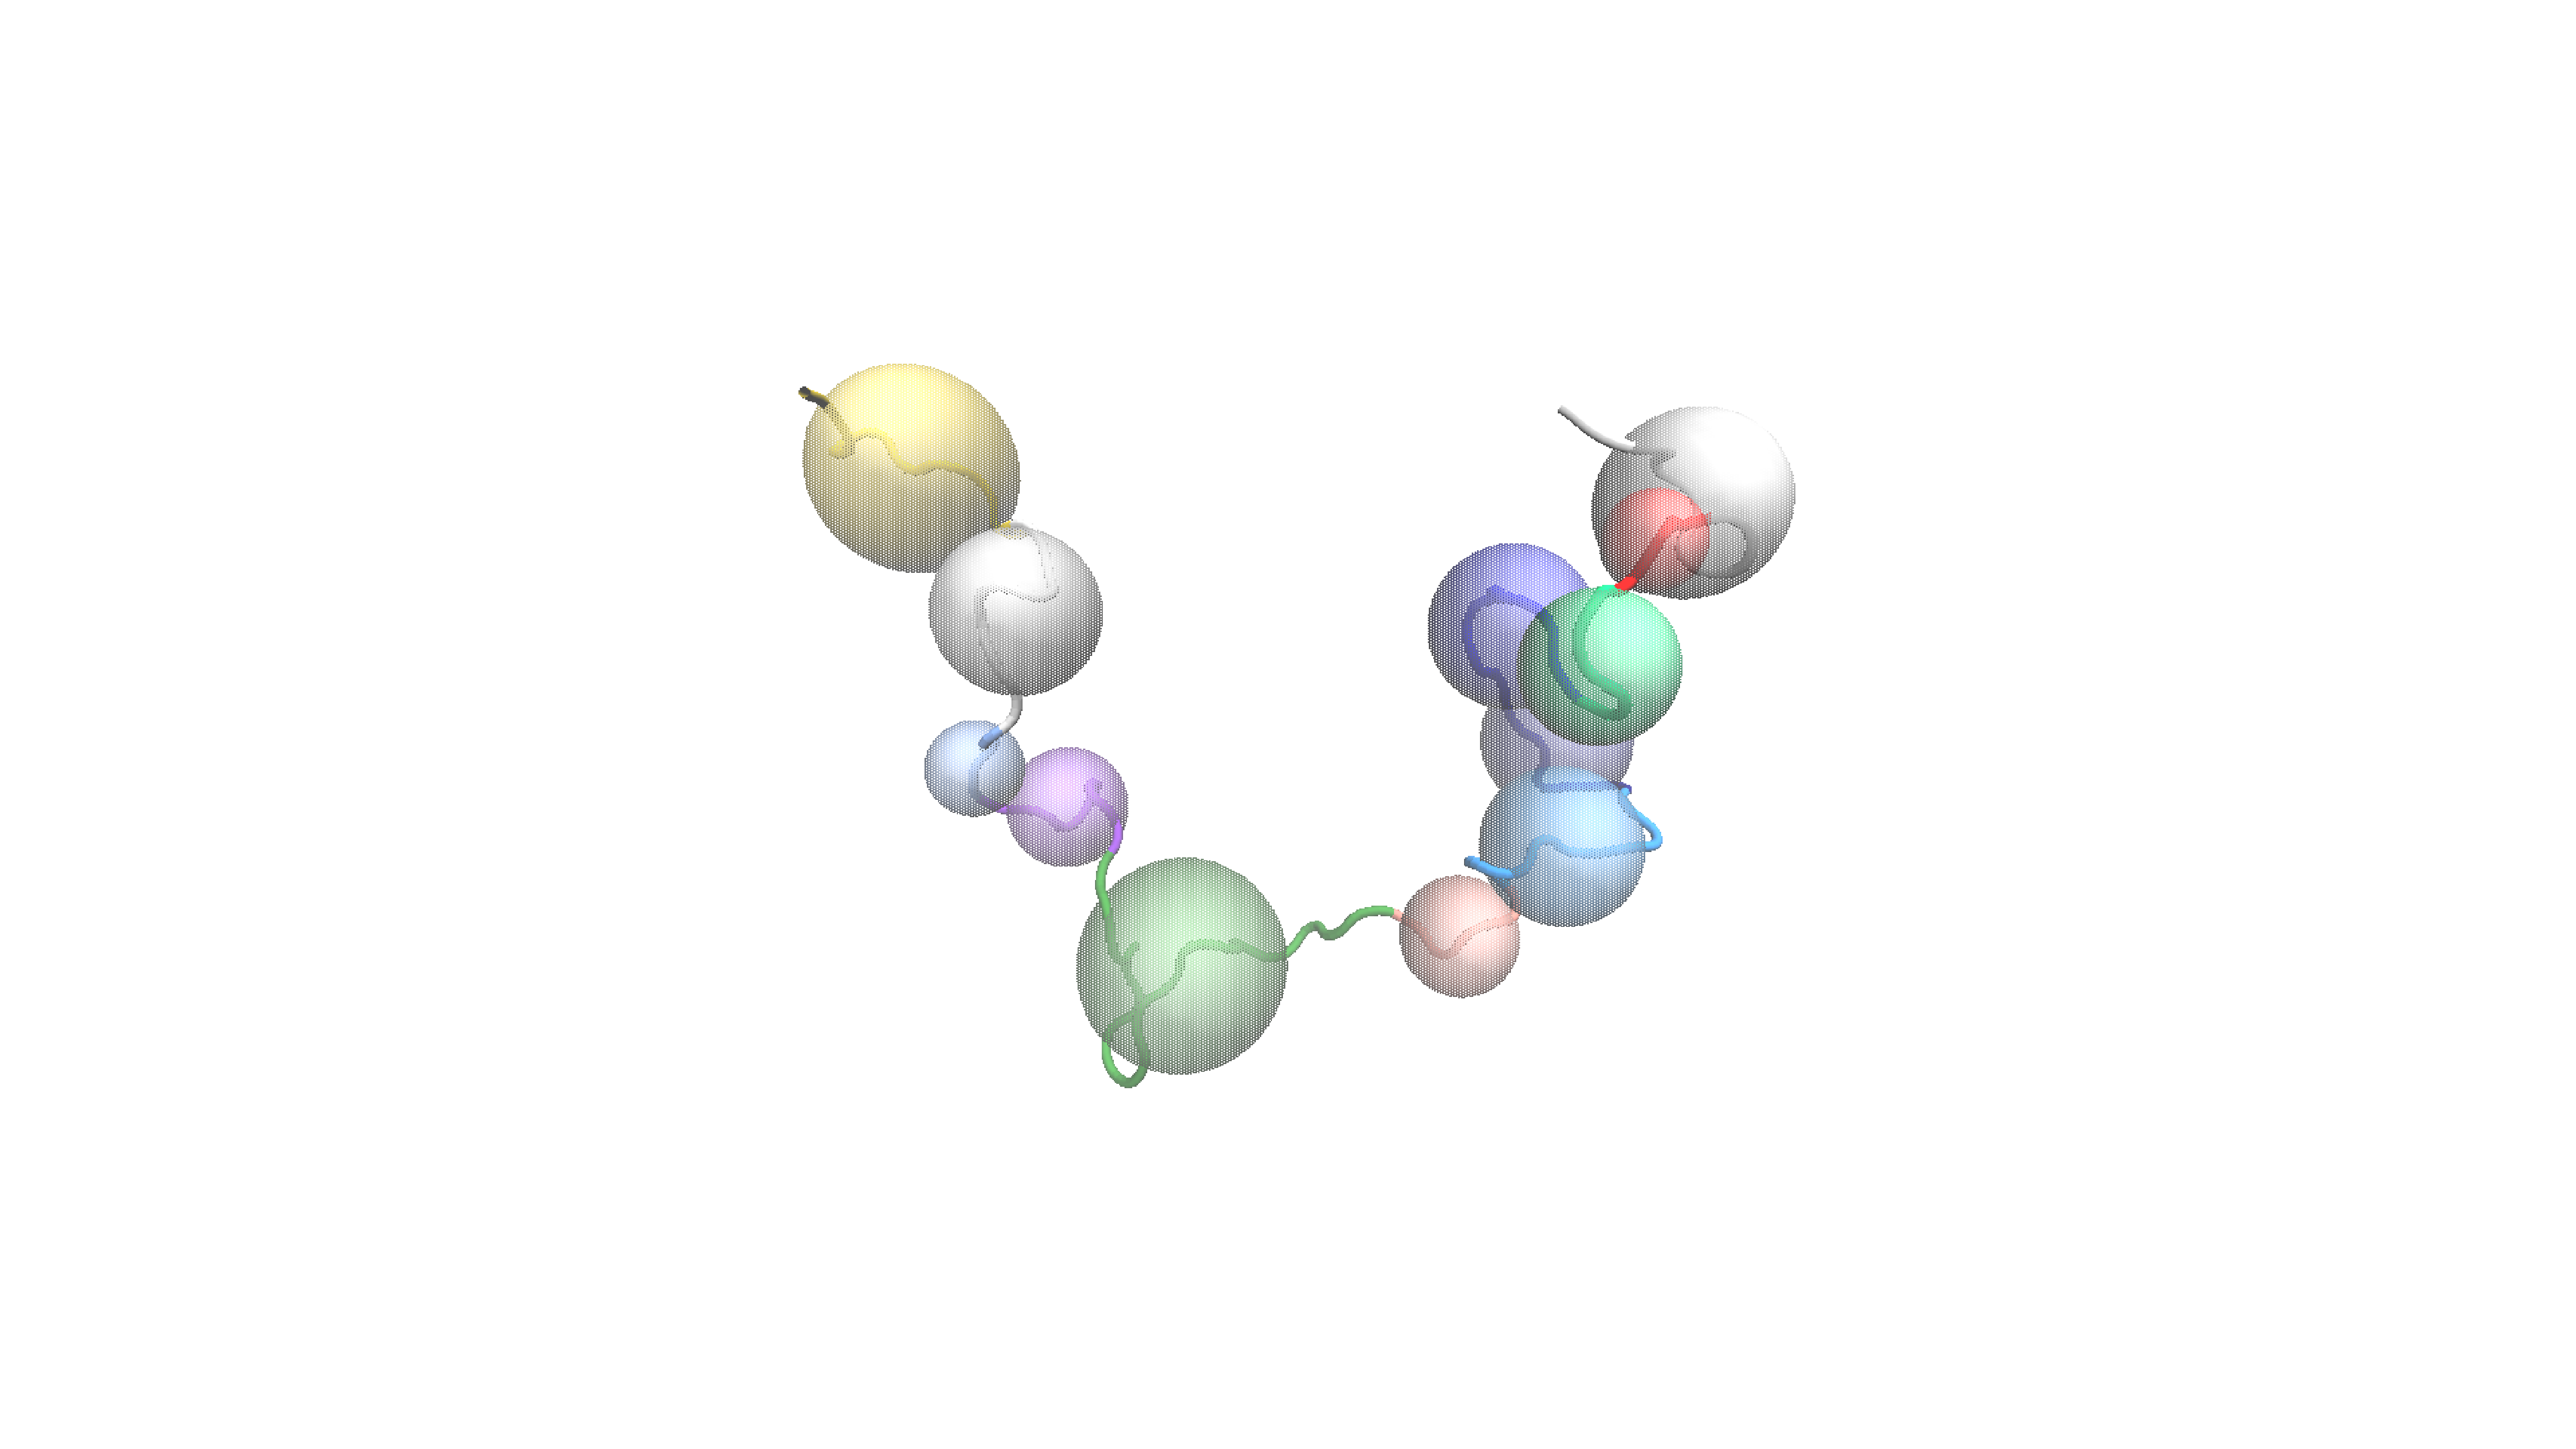
\includegraphics[width=0.5\textwidth, trim={35cm 18cm 35cm 18cm},clip]{MYC_all_beads.png}}
  \caption{\label{IDP_all_beads}The minimal assembly units of the 2 IDPs. The structures shown here are representatives selected from the trajectories with the lowest concentration of solute (0M urea for ACTR, 0.1M NaCl for MYC).}
\end{figure}

However, not like folded proteins who have a limited number of metastable states, the number of different simulations for IDPs can be very large. Thus, whether the increasing amount of data will lead to more and more assembly units or there will be an upper bound becomes a question worths investigation. To answer this question, we use only a part of the simulation data, and see how will the number of assembly units change as the amount of used data increases. In practical, with the coherent domains under all the conditions obtained by space time diffusion map, we calculate the average number of assembly units needed for all the possible combination of a sub-dataset with N simulations. The curves of average assembly units number against the size of the sub-dataset, N, is shown in fig-\ref{IDP_N_units}. 

While we didn't observe an obvious convergence of the assembly units number as the amount of used data increases. This may be caused by one of these two factors: 1) probably it's because the data we have is not enough, since there's a trend that the growth of assembly units number is slowing down as we use more simulations; 2) also, there might be no upper bound of the assembly units number for IDPs, because they have very different behaviors under different conditions. Whichever of these is true, it is sure that it's difficult to obtain a set of minimal assembly units works universally for IDPs, because it is either impossible or needs a large amount of data.

\begin{figure}[htbp]
  \centering
  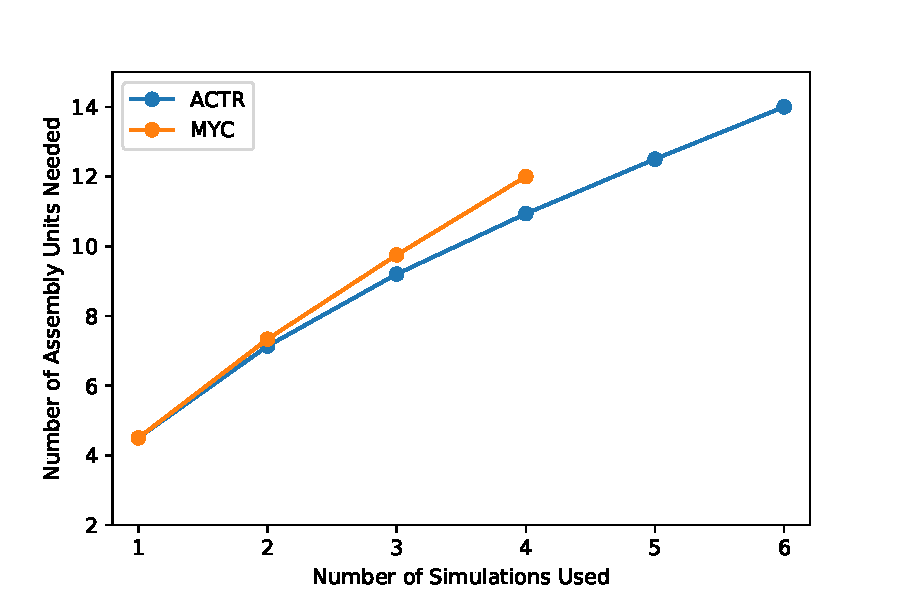
\includegraphics[width=1\textwidth]{IDP_N_units.pdf}
  \caption{\label{IDP_N_units}The average number of assembly units needed against the number of simulations used as dataset.}
\end{figure}

\section*{Conclusion}

By applying the {\it Structure and State Space Decomposition} algorithm\cite{Lrenzo_S3D} on a set of 10 fast-folding proteins, we confirmed the robustness of this algorithm. From the output results, we demonstrated that we can use a number of degrees of freedom which is smaller than $C_{\alpha}$ mapping to capture the long-timescale dynamics of proteins by appropriately making the selection of collective coordinates. For most proteins, their results show a consistency that the typical average size of the minimal assembly units locates between 20 to 30 heavy atoms, and for larger proteins this number will roughly become larger. However, if the dynamics of the protein is abnormal in some way, the decomposition result will also change coordinately.

Moreover, we also proposed a modified version of S3D for intrinsically disordered proteins, because their different dynamics makes Markov state model analysis inapplicable. As a result, we use the simulations under different conditions of IDPs as an analogue of the metastable states of folded proteins to complete the decomposition. However, because IDPs' behavior changes with the condition, we found as the number of input simulations grows more and more assembly units will be needed. We didn't observe an obvious convergence in this process. Thus, we conclude that it's difficult to find a set of minimal assembly units that works universally for IDPS.

Finally, as an outlook of this algorithm, since the minimal assembly units obtained with S3D is a good candidate of effective atoms for coarse-grained models, we hope we can develop a corresponding force filed so that a totally data-driven CG model can be constructed, which we believe will provide us a new perspective of view on coarse-grained modeling. For intrinsically disordered proteins, we can also construct such models by restricting the condition to control the number of assembly units. Furthermore, the decomposition result itself may also provide us inspirations on the relation between protein's structure and functions.

\section*{Acknowledgement}

We are grateful to D. E. Shaw Research and Dr. Zheng, Wenwei for sharing the simulation data used in the work. Wangfei want to thank all the members of Dr. Clementi's group for their help, especially for the introduction of S3D algorithm from Dr. Boninsegna, Lorenzo and the helpful discussions on TICA and Markov state model analysis with Dr. Feliks, Nüske. 

\clearpage

\bibliography{bib}

\bibliographystyle{Science}

% Your references go at the end of the main text, and before the
% figures.  For this document we've used BibTeX, the .bib file
% scibib.bib, and the .bst file Science.bst.  The package scicite.sty
% was included to format the reference numbers according to *Science*
% style.

% Following is a new environment, {scilastnote}, that's defined in the
% preamble and that allows authors to add a reference at the end of the
% list that's not signaled in the text; such references are used in
% *Science* for acknowledgments of funding, help, etc.

% For your review copy (i.e., the file you initially send in for
% evaluation), you can use the {figure} environment and the
% \includegraphics command to stream your figures into the text, placing
% all figures at the end.  For the final, revised manuscript for
% acceptance and production, however, PostScript or other graphics
% should not be streamed into your compliled file.  Instead, set
% captions as simple paragraphs (with a \noindent tag), setting them
% off from the rest of the text with a \clearpage as shown  below, and
% submit figures as separate files according to the Art Department's
% instructions.

\end{document}




















